%!TEX root = ..\..\main.tex
\chapter{Deconvolution}
\label{Ch:Deconvolution}

\lhead{Chapter \ref{Ch:Deconvolution}. \emph{Deconvolution}}

%-------------------------------------------------------------------------------
%	Chapter Text
%-------------------------------------------------------------------------------

% Quick summary of what Aurore said she expected the chapter to contain
% Explain basic deconvolution, phiU known
% PhiU est from replicates
% With no replicates brief summary of lit
% Delaigle Hall 2016
% Say authors noted few points of support
% Hard to come up with theoretical justification for why
% Here's empirical examples
% Looks like often need a lot less
% Motivates code with fewer parameters. This is faster.
% We do this in R-package.

\section{Introduction}
	In this final chapter, we look at another statistical problem in which we perform an optimization over discrete probability distributions and find that the number of points of support of the optimal distribution is much smaller than expected. In contrast to Chapter \ref{Ch:Mixtures}, we will take a descriptive and practically minded point of view, rather than the more theory driven previous chapter. This is partly due to the additional complexity of the problem, which prevents many of the tools used on maximum likelihood mixtures from working here. However, this does not stop us from pointing out similarities between the two problems, and an empirical exploration allows us to benefit from the similar phenomenon that occurs in a variety of scenarios
.
	The problem is one of \emph{deconvolution}, the recovery of the distribution, $F_X$, or density, $f_X$, of some random variable $X$, from measurements of
	\begin{equation}
		W = X + U
		\label{eq:W=X+U}
	\end{equation}
	where the measurement error $U$ is independent of $X$, and $U$ and $X$ are unobserved. %We use $\phi_X$ and $\phi_U$ to denote the characteristics functions of $X$ and $U$, and $F_X$ and $F_U$ for the distributions. We use $f_X$ and $f_U$ for the densities if they exist.

	In the case that we know the distribution of $U$, Carroll and Hall \cite{Carroll1988-aj} and Stefanski and Carroll \cite{Stefanski1990-uo} proposed a deconvolution kernel density estimator of $f_X$. If the distribution of $U$ is unknown, then it is often possible to estimate it from replicate measurements, $W_{jk} = X_j + U_{jk}$, for $1 \leq k \leq N_j$ and $1 \leq j \leq n$, where the $U_{jk}$'s are independent. Delaigle, Hall, and Meister provided an estimator for $f_X$ in this scenario. However, until Delaigle's and Hall's 2016 paper, ``Methodology for nonparametric deconvolution when the error distribution is unknown,'' \cite{Delaigle2016-la}, there had been no nonparametric method to estimate the distribution of $X$ when we had no data on the distribution of $U$ (see the discussion in Section 1 of \cite{Delaigle2016-la}).

	% [BRIEF SUMMARY OF LITERATURE]

	In this chapter, we focus on the methods introduced in \cite{Delaigle2016-la}. We will start in Section \ref{sec:summary of basic deconvolution} by summarizing deconvolution methods for the cases where the error distribution is known, or estimated from replicates. This will serve as a basis for a discussion of Delaigle's and Hall's \cite{Delaigle2016-la} paper in Section \ref{sec:summary of delaigle hall}. In Section \ref{sec:deconvolution empirical results}, we will empirically demonstrate that these methods produce a similar phenomenon to the one encountered in Chapter \ref{Ch:Mixtures} --- the probability mass function which we obtain from an optimization problem has only a few points of support ---  and we will explore how this phenomenon manifests under various conditions. We will also point out how we can take advantage of this phenomenon. 
	% Finally, in Section \ref{sec:deconvolution observations and results}, we will make some general observations about some similarities between our deconvolution problem, and that of maximum likelihood mixtures. 
	Finally, in Section \ref{sec:deconvolution observations and results}, we will make a general observation about the deconvolution problem, and point out some similarities between it and the mixture problem of Chapter \ref{Ch:Mixtures}.


\subsection{Prior deconvolution methods}
\label{sec:summary of basic deconvolution}
% \subsection{PhiU known}
	We start with the estimator of Stefanski and Carroll in \cite{Stefanski1990-uo}. In this scenario, we let $X$ and $U$ be independent random variables with probability density functions $f_X$ and $f_U$ respectively. We observe a set of $n$ independent observations, $\{W_j\}_{j = 1}^n$, where each $W_j$ is an observation of the $W$ of \eqref{eq:W=X+U}.
	Furthermore, we assume that $f_U$ is known. Given this information, the goal is to estimate $f_X$ from the $W_j$'s.

	The estimator makes use of characteristic functions. A random variable $Y$ with density $f_Y$ has characteristic function
	\begin{equation}
		\phi_Y(t) = \int_\mathbb{R} \euler^{i t x} f_Y(x) \intd x
	\end{equation}
	which can be inverted via
	\begin{equation}
		f_Y(x) = \frac{1}{2\pi} \int_\mathbb{R} \euler^{-itx} \phi_Y(t) \intd t
	\end{equation}
	if $\phi_Y$ is integrable. One property of characteristic functions that is convenient for this deconvolution problem is that since $X$ and $U$ are independent, we know that the characteristic function of $W = X+ U$ is
	\begin{equation}
		\phi_W = \phi_X \phi_U,
	\end{equation}
	or equivalently,
	\begin{equation}
		\phi_X = \frac{\phi_W}{\phi_U}
		\label{eq: phi_X is fraction phi_W phi_U}
	\end{equation}
	if $|\phi_U(t)| > 0$ for all real $t$. We assume this in constructing the following estimator.

	Let $K$ be a bounded, even, function that integrates to 1 whose Fourier transform, $\phi_K$, satisfies
	\begin{align}
		\sup_t |\phi_K(t) / \phi_U(t / h) | < \infty, &&\int_\mathbb{R} |\phi_K(t) / \phi_U(t / h)| \intd t < \infty,
		\label{eq:phiK conditions error known}
	\end{align}
	for any fixed $h > 0$ (we impose these conditions to make various functions integrable). We may estimate the density of $W$ via the usual kernel density estimator \cite[Section 20.3]{Wasserman2003-ot}
	\begin{equation}
		\hat{f}_W(x) = \frac{1}{n h} \sum_{j = 1}^n K((x - W_j)/h),
	\end{equation}
	which has characteristic function
	\begin{equation}
		\hat{\phi}_W(t) = \phi_{W_\mathrm{EMP}}(t) \phi_K(h t)
	\end{equation}
	where $\phi_{W_\mathrm{EMP}}(t)$ denotes the empirical characteristic function of $\{W_j\}_{j = 1}^n$,
	\begin{equation}
		\phi_{W_\mathrm{EMP}}(t) = \frac{1}{n}\sum_{j = 1}^n \euler^{itW_j}.
	\end{equation}

	Motivated by \eqref{eq: phi_X is fraction phi_W phi_U}, we may estimate the characteristic function of $X$ by 
	\begin{equation}
		\hat{\phi}_X = \hat{\phi}_W / \phi_U
	\end{equation}
	and the density of $X$ by inverting $\hat{\phi}_X$. Overall, the estimator for $f_X$ is given by
	\begin{equation}
	\label{eq:standard deconvolution estimator}
		\hat{f}_X(x) = \frac{1}{2\pi} \int_\mathbb{R} \euler^{-itx} \phi_K(ht) \phi_{W_\mathrm{EMP}}(t)  / \phi_U(t) \intd t.
	\end{equation}

% \subsection{PhiU est from replicates}
	If the distribution of $U$ is unknown, it is often possible to estimate it if replicate measurements are present. Methods for deconvolution with the presence of replicates have been presented in \cite{Li1998-mj}, \cite{Lin2006-mm}, \cite{Delaigle2008-hl}, and also \cite{McIntyre2011-fg} in the case of heteroscedastic errors. Here we look at the estimator of Delaigle, Hall, and Meister \cite{Delaigle2008-hl} as it has the most similarities with the estimator of interest in this chapter.

	In this setting, we measure
	\begin{align}
		W_{jk} = X_j + U_{jk} && j = 1, \dots, n \text{ and } k = 1, \dots, N_j
	\end{align}
	where the $X_j$ and $U_{jk}$ are independent and are identically distributed as $X$ and $U$ respectively. A consistent estimator of $\phi_U(t)$ is
	\begin{equation}
		\hat{\phi}_U(t) = \left|\frac{1}{N} \sum_{j = 1}^n \sum_{(k_1, k_2) \in \mathscr{S}_j} \cos \left(t (W_{jk_1} - W_{jk_2})\right)\right|^{1/2},
		\label{eq:phi_U estimator}
	\end{equation}
	where $\mathscr{S}_j$ is the set of $N_j(N_j - 1)/2$ pairs $(k_1, k_2)$ with $1 \leq k_1 < k_2 \leq N_j$, and $N = \sum_{j=1}^n N_j(N_j - 1)/2$ is the total number of terms inside \eqref{eq:phi_U estimator}.
	%
	In light of \eqref{eq:standard deconvolution estimator}, this suggests an estimator of $f_X$ given by 
	\begin{equation}
	\label{eq:replicates estimator}
		\hat{f}_X(x) = \frac{1}{2\pi} \int_\mathbb{R} \euler^{-itx} \phi_K(ht) \phi_{W_\mathrm{EMP}}(t)  / (\hat{\phi}_U(t) + \rho )\intd t
	\end{equation}
	with
	\begin{equation}
		\phi_{W_\mathrm{EMP}}(t) = \frac{1}{M} \sum_{j = 1}^n \sum_{k= 1}^{N_j} \euler^{i t W_{jk}}
	\end{equation}
	where
	% \begin{equation}
	% 	\hat{f}_X(x) = \frac{1}{Mh} \sum_{j = 1}^n \sum_{k = 1}^{N_j} \hat{L}\left(\frac{x - W_{jk}}{h}\right)
	% \end{equation}
	% where
	% \begin{equation}
	% 	\hat{L}\left(u\right) = \frac{1}{2\pi} \int \euler^{-itu} \phi_K(t) / (\hat{\phi}_U(t/h) + \rho) \intd t,
	% \end{equation}
	$h > 0$ is a bandwidth, $\rho \geq 0$ is a ridge parameter (which we explain below), $M = \sum_j N_j$, and $K$ is a symmetric kernel function, whose Fourier transform, $\phi_K$, has compact support. As in \eqref{eq:phiK conditions error known}, this last condition is to make sure that an integral (in this case, \eqref{eq:replicates estimator}) converges. The condition is stronger than \eqref{eq:phiK conditions error known} since the error distribution is unknown and so we have to account for more possibilities.

	% [WHY COMPACT SUPPORT?]

	The presence of the ridge parameter is to account for potential fluctuations in $\hat{\phi}_U$ that could cause the denominator in \eqref{eq:replicates estimator} to be zero, or too close to zero. We may alternatively use another method to prevent $\hat{\phi}_U(t)$ from getting too close to zero such as replacing $\hat{\phi}_U(t)$ with some other function for $|t|$ larger than some threshold $t^*$.

	A similar approach could be used in scenarios where we are able to sample directly from the distribution of $U$. See also \cite{Diggle1993-jy} and \cite{Neumann1997-cr} for further discussion of cases where samples of the errors are available.

	% \subsection{U unknown}
	In the case where we do not know the distribution of $U$, nor have access to replicate measurements or direct measurements from $U$, methods for deconvolution generally require $F_U$ to have a parametric or semi-parametric form. Such methods can be found in \cite{Butucea2005-be}, \cite{Meister2006-nu}, \cite{Butucea2008-wm}, and \cite{Kneip2012-aa}. One exception to this is found in \cite{Schennach2013-yv} where the authors discuss non-parametric estimation of an errors-in-variables regression problem without extra information about the error distributions. However, in regression problems one has access to not only observations of $W = X+ U$, but also observations of $Y = g(X) + \epsilon$, where $\epsilon$ denotes some independent experimental error. This extra data contains information about $F_U$ which, at least in theory, makes it easier to estimate than in the plain deconvolution case.
 
\section{Method for deconvolution when the error is unknown}
\label{sec:summary of delaigle hall}
	Delaigle's and Hall's 2016 paper \cite{Delaigle2016-la}, presents a non-parametric deconvolution estimator for when the error distribution is unknown, and we do not have access to replicates or samples from the error distribution. %This is unusual in deconvolution problems. As in the methods described above, deconvolution methods usually require assumptions about the shape or scale of the error distribution, or rely on additional observations to estimate it. 
	In this section we summarise the estimator of \cite{Delaigle2016-la}, and discuss some practicalities that arise in the implementation. 

	\subsection{Problem Setup}
	Suppose that we observe $(W_1, \dots, W_n)$, where
	\begin{align}
		W_j &= X_j + U_j &&j = 1, \dots, n
	\end{align}
	and $X_j$ and $U_j$ are independent and identically distributed as $X$ and $U$ respectively, and $X$ and $U$ are independent. 

	% Suppose also that we do not know any information concerning the distribution of $U$. This is unusual in deconvolution problems; we usually assume that we either know the distribution of $U$, at least up to a scaling factor, or that replicate measurements of the $W_j$s are available for the same $X_j$. 

	We need the following assumptions about $U$ and its characteristic function, $\phi_U$:
	\begin{assumption}
	\label{assump:phiU real}
		$\phi_U$ is real-valued.
	\end{assumption}
	\begin{assumption}
	\label{assump:phiU non zero}
		For $U$ discrete, $\phi_U$ is non-negative and is zero at at most a countable number of points, and for $U$ continuous, $\phi_U$ is strictly positive on the whole real line.
	\end{assumption}

	Assumption \ref{assump:phiU real} is equivalent to assuming that the distribution of $U$ is symmetric. Assumption \ref{assump:phiU non zero} is a standard assumption in deconvolution problems. These conditions are mild and some common distributions which satisfy them when centred around zero include the normal distribution, the Laplace distribution, and the Cauchy distribution.

	% [WHAT DOES $\phi_U \geq 0$ MEAN FOR $f_U$]

	We also make the following assumptions on the distribution of $X$:
	% We write the convolution of distributions $F$ and $G$ as
	% \begin{equation}
	% 	(F \circ G)(x) = \int F(x - u) \intd G(u).
	% \end{equation}
	\begin{assumption}
	\label{assumpt: X not symmetric}
		$F_X$ is not symmetric.
	\end{assumption}
	\begin{assumption}
		\label{assump: X indecomposable}
		It is not possible to decompose $X$ as
		\begin{equation}
			X = Y + Z
		\end{equation}
		for nondegenerate and independent random variables $Y$ and $Z$ with $F_Z$ symmetric.
	\end{assumption}

	We require these assumptions because all we know about $F_U$ is that it is symmetric. So if $F_X$ was also symmetric, we could not distinguish it from $F_U$, and if $X$ is itself made up of a symmetric part $Z$, we could not distinguish $U$ from $Z+U$.


	To form the estimator for $F_X$, we will make use of the \emph{phase function}, which for a random variable $V$, is defined by
	\begin{equation}
		\rho_V = \frac{\phi_V}{|\phi_V|}
	\end{equation}
	on all points where $\phi_V \neq 0$.
	Note that from Assumption \ref{assump:phiU real}, we have that 
	\begin{equation}
	\label{eq: phiU equal mod phiU}
		\phi_U = |\phi_U|
	\end{equation}
	and so $\rho_U = 1$.
	Since $W = X+U$, with $X$ and $U$ independent, we have that
	\begin{align}
		\phi_W = \phi_X \phi_U
	\end{align}
	and so from \eqref{eq: phiU equal mod phiU}, on all points where $\phi_U \neq 0$,
	\begin{align}
		\rho_W = \rho_X.
	\end{align}
	In fact, all random variables of the form $V = X + Z$, where $Z$ is symmetric and independent of $X$, will have phase function $\rho_W$, and the variance of these will satisfy $\var(V) \geq \var(X)$. This motivates the final assumption we make for $X$:

	\begin{assumption}
	\label{assump:X has smallest variance}
		$F_X$ has the uniquely smallest variance out of all distributions with phase function $\rho_X$.
	\end{assumption}

	\subsection{Estimator}
	\label{sec:deconvolution estimator}
	From the discussion above, we might think to take our estimator for $F_X$ to be the distribution that has smallest variance out of all distributions with phase function equal to some estimator of $\rho_W$ constructed from $W_1, \dots, W_n$. However, when it comes to the implementation of our estimator, there are some additional details which make it more complex. We will introduce these details by presenting a hierarchy of estimators, leading from the idealised problem to what we implement in practice. 

	\subsubsection{Estimator 1}
	As mentioned above, ideally we would like to $\hat{F}_X$ to be the distribution with smallest variance out of all distributions with phase function equal to some estimator of $\rho_W$. We can estimate $\rho_W$ by
	\begin{equation}
		\hat{\rho}_W = \frac{\hat{\phi}_W}{\left|\hat{\psi}_W\right|^{1/2}}
	\end{equation}
	where
	\begin{equation}
	\label{eq:define hat phi W}
		\hat{\phi}_W(t) = \frac{1}{n}\sum_{j = 1}^n \exp(it W_j)
	\end{equation}
	and 
	\begin{equation}
	\label{eq:define hat psi W}
		\hat{\psi}_W(t) = \frac{1}{n(n-1)} \sum_{k=1}^n \sum_{j \neq k} \exp(it (W_j - W_k))
	\end{equation}
	are consistent estimators of $\phi_W$ and $\psi_W = |\phi_W|^2$ respectively. This gives us our first estimator,
	\begin{equation}
		\hat{F}_X^1 = \argmin_{F \in \mathscr{F}_1} \var(F),
	\end{equation}
	where 
	\begin{equation}
		\mathscr{F}_1 = \{F: \rho_F(t) = \hat{\rho}_W(t), \forall t \in \mathbb{R}\}
	\end{equation}
	is the set of distributions with phase function equal to $\hat{\rho}_W$.

	\subsubsection{Estimator 2}
	% Ideally, we would like to choose our estimate for $F_X$ to have phase function $\hat{\rho}_X = \hat{\rho}_W$, or equivalently, $\hat{\phi}_W(t) |\hat{\phi}_X(t)| - |\hat{\phi}_W(t)| \hat{\phi}_X(t) = 0$ for all $t$. 
	% However, unless we take $F_X$ to be the empirical distribution function of $\{W_j\}_j$, it is not clear that it is even possible to choose it to have phase function exactly equal to $\hat{\rho}_W$. 
	However, $\hat{\rho}_W(t)$ grows less reliable for large values of $|t|$, and so we should preference matching $\hat{\rho}_X$ and $\hat{\rho}_W$ around $t = 0$ over large values of $|t|$. Furthermore, it is not clear that there even exists a distribution with phase function equal to $\hat{\rho}_W(t)$ for all $t \in \mathbb{R}$. Taking this into consideration, and noting that when $\rho_F(t) = \hat{\rho}_W(t)$ we have $\hat{\phi}_W(t) |\phi_F(t)| - \left|\hat{\psi}_W(t)\right|^{1/2} \phi_F(t) = 0$, our goal is to instead choose an $F$ that makes
	\begin{equation}
		T(F) = \int_{-\infty}^\infty \left| \hat{\phi}_W(t) |\phi_F(t)| - \left|\hat{\psi}_W(t)\right|^{1/2} \phi_F(t) \right|^2 w_1(t) \intd t
	\end{equation}
	small,
	where $w_1(t)$ is some non-negative symmetric weight function that assigns greater weight when $|t|$ is small. This gives us our second estimator.
	Find 
	\begin{equation}
		T^\mathrm{min} = \min_F T(F)
	\end{equation}
	and put
	\begin{equation}
		\hat{F}_X^2 = \argmin_{F \in \mathscr{F}_2} \var{F},
	\end{equation}
	where
	\begin{equation}
		\mathscr{F}_2 = \{F: T(F) = T^\mathrm{min}\}.
	\end{equation}

	\subsection{Estimator 3}

	A concern that we might have at this stage is that even though $\phi_U = \phi_W / \phi_X$, there is no guarantee that 
	\begin{equation}
		\hat{\phi}_U = \hat{\phi}_W / \phi_{\hat{F}}
	\end{equation}
	is a valid characteristic function, or that it is real-valued as per Assumption \ref{assump:phiU real}.
	% We also expect that $\hat{\phi}_U = \hat{\phi}_W / \phi_F$ should be real-valued as per Assumption \ref{assump:phiU real}, and have magnitude less than or equal to 1 as all characteristic functions do. 
	For $\hat{\phi}_U$ to be real-valued we require that
	\begin{equation}
		\Im \left( \frac{\hat{\phi}_W}{\phi_F} \right) = 0
	\end{equation}
	where we use $\Im(z)$ to denote the imaginary part of $z$. Using $\bar{z}$ to denote the complex conjugate of $z$, we can replace this by,
	\begin{equation}
		\Im \left(\frac{\hat{\phi}_W \bar{\phi}_F}{|\phi_F|^2} \right) = 0,
	\end{equation}
	or again,
	\begin{equation}
		\Im \left(\hat{\phi}_W \bar{\phi}_F\right) = 0.
	\end{equation}
	In an attempt to satisfy this, we construct a penalty
	% We try to satisfy this by constructing penalties which we desire to be small,
	\begin{align}
		P_1(F) = \int \Im \left(\hat{\phi}_W \bar{\phi}_F\right) w_2(t)\intd t,
		\label{eq:penalty1}
	\end{align}
	which we desire to be small,
	where $w_2(t)$ is some non-negative symmetric weight function with bounded support.	

	It is difficult to determine whether a given function is a characteristic function, but we can at least try to force $\hat{\phi}_U$ to have magnitude less than or equal to 1, as all valid characteristic functions do. We use the penalty
	\begin{align}
		P_2(F) = \int \left(|\hat{\phi}_U(t)| - 1\right) \indicator_{\{|\hat{\phi}_U(t)| > 1\}}  w_2(t) \intd t.
		\label{eq:penalty2}
	\end{align} 

	Overall, our third estimator, and the one we use in practice, is as follows. Let $\mathscr{F}$ be the set of distributions over which we search for our estimator (for example, discrete distributions with no more than $m$ points of support). Find
	\begin{equation}
		F_0 = \argmin_{F \in \mathscr{F}} \left[T(F) + \lambda_1 P_1(F) + \lambda_2 P_2(F)\right],
		\label{eq:objective 1}
	\end{equation}
	for some choice of scaling factors $\lambda_1$ and $\lambda_2$, and set
	\begin{align}
		T^\mathrm{min} &= T(F_0)\\
		P_1^\mathrm{min} &= P_1(F_0)\\
		P_2^\mathrm{min} &= P_2(F_0).
	\end{align}
	Then our estimator for $F_X$ is
	\begin{equation}
		\hat{F}_X = \argmin_{F \in \mathscr{F}} \var{F}
		\label{eq:objective 2}
	\end{equation}
	subject to the constraints $T(F) \leq T^\mathrm{min}$, $P_1(F) \leq P_1^\mathrm{min}$, and $P_2(F) \leq P_2^\mathrm{min}$.

	The idea behind these constraints is that, ideally, we want $T(F) = P_1(F) = P_2(F) = 0$ but cannot achieve this in practice. So instead, in our first optimization, we search for a more reasonable set of values to which we should restrict them. One might expect that $F_0$ is the only distribution which satisfies these constraints, and so we would always find that $\hat{F}_X = F_0$. However, in practice, we have not observed this. Either our first optimization does not find the global minimum, or there are multiple distributions which attain the minimum values for $T$, $P_1$, and $P_2$. One might also choose to replace $T^\mathrm{min}$ with $T^\mathrm{min}(1 + \delta)$ for some small $\delta$ (and similarly for $P_1^\mathrm{min}$ and $P_2^\mathrm{min}$) so that we are searching over a larger space in \eqref{eq:objective 2}.
	
	
	% [UP TO HERE ]

	% In practise, we perform this minimization over some set of distributions $F$ (for example, discrete distributions with no more than $m$ points of support). Call this set $\mathscr{F}$. Having found
	
	% we then choose our estimator to be the distribution $F \in \mathscr{F}$ that has smallest variance, under the constraint that $T(F) = T_\mathrm{min}$.

	\subsection{Numerical Implementation}

	Delaigle and Hall \cite{Delaigle2016-la} suggested performing this optimization problem by approximating $F_X$ with a discrete distribution on $m$ points, allowing $m$ potentially to diverge with the sample size. They suggested choosing the locations of the probability masses of that discrete distribution, $\vect{\theta} = (\theta_1, \dots, \theta_m)$, to be distributed uniformly but randomly along $[\min(W_i), \max(W_i)]$ and letting the corresponding probability weights $\vect{p} = (p_1, \dots p_m)$ be the variables over which we find the solution of \eqref{eq:objective 1} -- \eqref{eq:objective 2}. We will denote by $F_{\vect{\theta}, \vect{p}}$ the distribution that places mass $p_j$ at $\theta_j$ for $j = 1,\dots, m$. Its characteristic function is given by
	\begin{equation}
		\phi_{\vect{\theta}, \vect{p}}(t) = \sum_{j = 1}^m p_j \exp(it\theta_j)
	\end{equation}
	and its phase function by
	\begin{equation}
		\rho_{\vect{\theta}, \vect{p}}(t) = \frac{ \sum_{j = 1}^m p_j \exp(it\theta_j)}{\left| \sum_{j = 1}^m p_j \exp(it\theta_j)\right|}.
	\end{equation}
	It has variance
	\begin{equation}
		\var(F_{\vect{\theta}, \vect{p}}) = \sum_{j = 1}^m p_j \theta_j^2 - \left( \sum_{j=1}^m p_j \theta_j \right)^2.
	\end{equation}

	For the weight function, $w_1(t)$, Delaigle and Hall \cite{Delaigle2016-la} used the Epanechnikov kernel, rescaled to an interval $[-t^*, t^*]$. To choose $t^*$, they pointed out that since $\hat{\phi}_W$ is an unbiased estimator for $\phi_W$, and since it has variance no more than $1/n$, we can expect it to be a reasonable estimator when $|\hat{\phi}_W(t)| \geq n^{-1/4}$. They therefore chose $t^*$ to be the smallest $t > 0$ such that 
	\begin{equation}
	\label{eq:define t star}
		\left|\hat{\phi}_W(t)\right| \leq n^{-1/4}.
	\end{equation}
	For the weight function in the penalty terms, they used $w_2(t) = \indicator_{\{|t| \leq t^*\}}$. They used $\lambda_1 = \lambda_2 = 500 \Delta t$ for the scaling factors in \eqref{eq:objective 1}, where $\Delta t$ is the distance between grid points in their approximation of the integrals in \eqref{eq:penalty1} and \eqref{eq:penalty2}.
	There is some freedom of choice in the number of points in the approximating discrete distribution but the authors suggested that in their experience, $m = 5\sqrt{n}$ is a reasonable choice.

	\subsection{Example}
	In Figure \ref{fig:fixed masses example no smoothing}, we provide an example of a typical output of the method just described. In this example we have sampled $n = 500$ points of $W = X+U$ where the true distribution, $F_X$, is chi-squared with 3 degrees of freedom, rescaled to have variance $\sigma_X^2 = 1$. The error distribution, $F_U$, is normal with variance $\sigma_U^2 = 0.2$, resulting in a noise to signal ratio (NSR) of $0.2$. Our deconvolved estimator, $\hat{F}_{\vect{\theta}, \vect{p}}$, is represented by placing a grey point at each $(\theta_j, p_j)$. For comparison, we also plot the true density, $f_X(x)$, as well as an empirical kernel density estimator of $f_W$.

	\begin{figure}[ht]
		\centering
		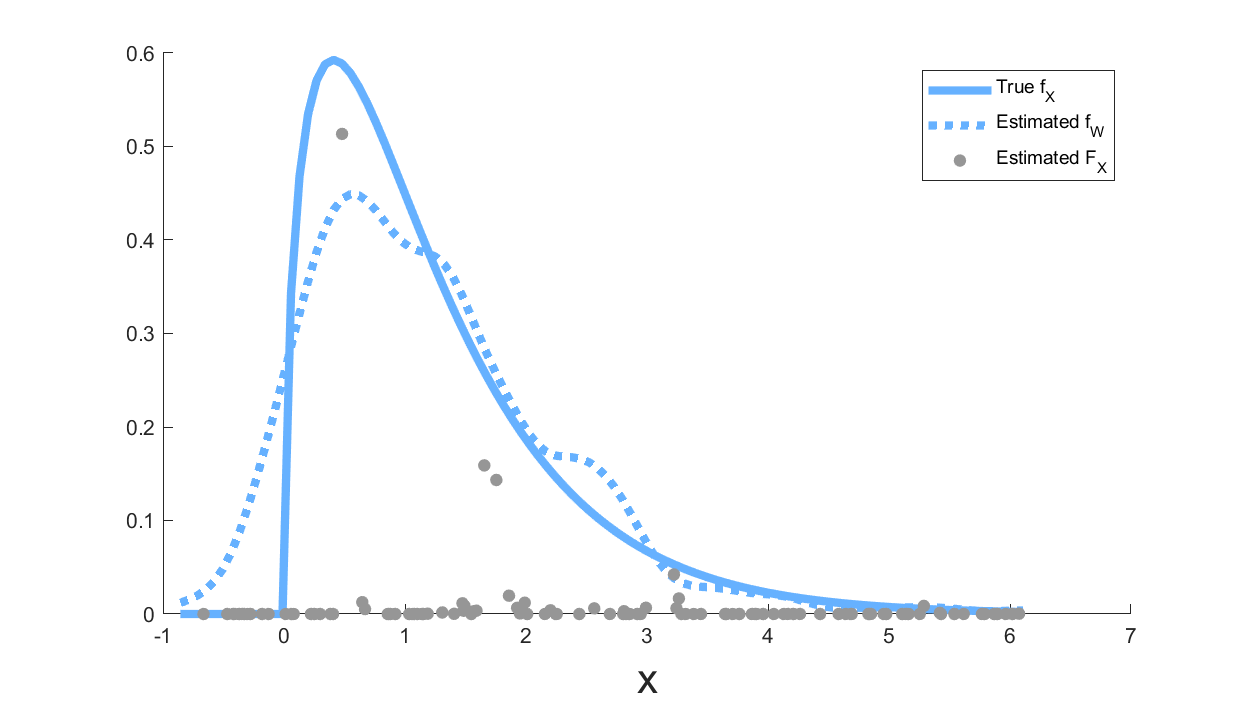
\includegraphics[width = \textwidth]{Figures/Deconvolution/fixed_masses_example_nosmoothing.png}
		\caption{A typical deconvolution following the method of Delaigle and Hall \cite{Delaigle2016-la}.}
		\label{fig:fixed masses example no smoothing}
	\end{figure}

	There are two things we wish to highlight here. The first is that the majority of the probability weights $p_j$ are either close to or equal to zero. Only a select few points seem to contribute notably to the estimator. This is reminiscent of Figure \ref{fig:collapsing distribution} in which most of the probability masses in the unsimplified mixing distribution were redundant. This phenomenon appears consistently over a wide variety of deconvolution problems and we will explore this further in Section \ref{sec:empirical results}. 

	The second point we want to highlight is that it is hard to compare our discrete estimator with the continuous true density. Based on Figure \ref{fig:fixed masses example no smoothing} alone, one might even say that $\hat{F}_{\vect{\theta},\vect{p}}$ is a very poor estimator for $F_X$. So we now describe how we can construct a continuous estimator from the discrete one. This continuous estimator will allow us to more intuitively evaluate how well our deconvolution has performed.

	% Delaigle and Hall also impose some additional constraints. We desire that 
	% \begin{equation}
	% 	\hat{\phi}_U = \frac{\hat{\phi}_W}{\phi_{\vect{\theta}, \hat{\vect{p}}}}
	% \end{equation}
	% is both symmetric (to be consistent with Assumption \ref{assump:phiU real}) and satisfies $\hat{\phi}_U(t) \leq 1$ (as all characteristic functions must satisfy this). In \cite{Delaigle2016-la}, these are stated as hard constraints, however in practise [CITE CODE OR CORREPONDENCE], these are added via penalty terms to $T(F)$.

	% Overall, the final method is as follows.

	% \begin{enumerate}
	% 	\item Set $m = 5\sqrt{n}$ and fix $\vect{\theta} = (\theta_1, \dots, \theta_m)$ to be distributed uniformly at random along $[\min(W_i), \max(W_i)]$.
	% 	% \item 
	% 	\item Define $\hat{\phi}_W$ and $\hat{\psi}_W$ as in \eqref{eq:define hat phi W} and \eqref{eq:define hat psi W}.
	% 	\item Define $t^*$ as in \eqref{eq:define t star}.
	% 	\item Define
	% 	\begin{equation}
	% 		T(F_{\vect{\theta}, \vect{p}}) = \int_{-t^*}^{t^*} \left| \hat{\phi}_W(t) - \left|\hat{\psi}_W(t)\right|^{1/2} \frac{ \sum_{j = 1}^m p_j \exp(it\theta_j)}{\left| \sum_{j = 1}^m p_j \exp(it\theta_j)\right|} \right|^2 w(t) \intd t.
	% 	\end{equation}
	% 	where $w(t)$ is the Epanechnikov kernel rescaled to $[-t^*, t^*]$.
	% 	\item
	% 	Calculate
	% 	\begin{equation}
	% 		 \vect{p}' = \argmin_{\vect{p}} \left\{T(F_{\vect{\theta}, \vect{p}}) + \mathrm{penalties}(\vect{p})\right\}
	% 	\end{equation}
	% 	and set
	% 	\begin{align}
	% 		T_\mathrm{min} &= T(F_{\vect{\theta}, \vect{p}'})\\
	% 		\mathrm{penalties}_\mathrm{min} &= \mathrm{penalties}(\vect{p}')
	% 	\end{align}
	% 	\item Calculate
	% 	\begin{equation}
	% 		\hat{\vect{p}} = \argmin \left\{ \sum_{j = 1}^m p_j \theta_j^2 - \left( \sum_{j=1}^m p_j \theta_j \right)^2 \right\}
	% 	\end{equation}
	% 	subject to
	% 	\begin{equation}
	% 		T(F_{\vect{\theta}, \vect{p}}) \leq T_\mathrm{min}
	% 	\end{equation}
	% 	and 
	% 	\begin{equation}
	% 		\mathrm{penalties} \leq \mathrm{penalties}_\mathrm{min}
	% 	\end{equation}
	% 	\item The final estimator for $F_X$ is $\hat{F}_X = F_{\vect{\theta}, \hat{\vect{p}}}$.
	% \end{enumerate}
	% [BE MORE PRECISE ABOUT PENALTIES?]


	% [DIFFERENT DEFINITION FOR T(P) THAT AURORE USES (AND NOW ME TOO)]

	\subsection{Converting to continuous distribution}

	If $X$ is continuous, then we will often want to use $\hat{F}_X = F_{\vect{\theta}, \vect{p}}$ to create an estimate of the density, $f_X$. Perhaps the most obvious solution is to use
	\begin{equation}
		\hat{f}_X(x) = \sum_{j=1}^m p_j K((x - \theta_j)/h)
	\end{equation}
	where $K$ is a kernel and $h > 0$ is a bandwidth. This is exactly equivalent to 
	\begin{equation}
		\hat{f}_X(x) = \frac{1}{2\pi}\int_{-\infty}^{\infty} \euler^{-itx} \phi_{\vect{\theta}, \vect{p}}(t) \phi_K(ht) \intd t
	\end{equation}
	where $\phi_K$ is the Fourier transform of $K$. However, since we only used $t \in [-t^*, t^*]$ when constructing $\phi_{\vect{\theta}, \vect{p}}$, it is reasonable to assume that $\phi_{\vect{\theta}, \vect{p}}(t)$ is less reliable for $t$ outside this range. This motivates replacing $\phi_{\vect{\theta}, \vect{p}}(t)$ with
	\begin{equation}
		\tilde{\phi}(t) = 
		\begin{cases}
			\phi_{\vect{\theta}, \vect{p}}(t), & t \in [-t^*, t^*],\\
			r(t), & \text{otherwise},
		\end{cases}
	\end{equation}
	where $r(t)$ is some ridge function. Delaigle and Hall \cite{Delaigle2016-la} suggest following \cite{Delaigle2008-hl} and using
	\begin{equation}
		r = \hat{\phi}_W / \hat{\phi}_{U,P}
	\end{equation}
	where $\hat{\phi}_{U,P}$ is the characteristic function of a Laplace distribution with variance equal to an estimator of the variance of $U$, obtained as a by-product of their estimator of $\phi_U$. They also suggest choosing the bandwidth, $h$, using the two-stage plug-in bandwidth of Delaigle and Gijbels \cite{Delaigle2002-pa} \cite{Delaigle2004-fy}. This method requires that $\phi_U$ is known, however, we may simply replace it by its estimator,
	\begin{equation}
		\hat{\phi}_U(t) = \frac{|\hat{\phi}_W|}{|\hat{\phi}_{\vect{\theta},\vect{p}}|}.
	\end{equation}

	% [as if $f_U$ was known, just replacing it by its estimator.]

	% [EXPLAIN WE GET ON ESTIMATOR OF $\phi_U$ FROM THIS TECHNIQUE AND SAY HOW TO GET IT]

	In Figure \ref{fig:fixed masses example alone} we add our continuous estimator, $\hat{f}_X(x)$, to the results from Figure \ref{fig:fixed masses example no smoothing}. Now it is easy to visually confirm that our estimator has indeed improved upon the empirical kernel density estimator for $f_W$.

	\begin{figure}
		\centering
		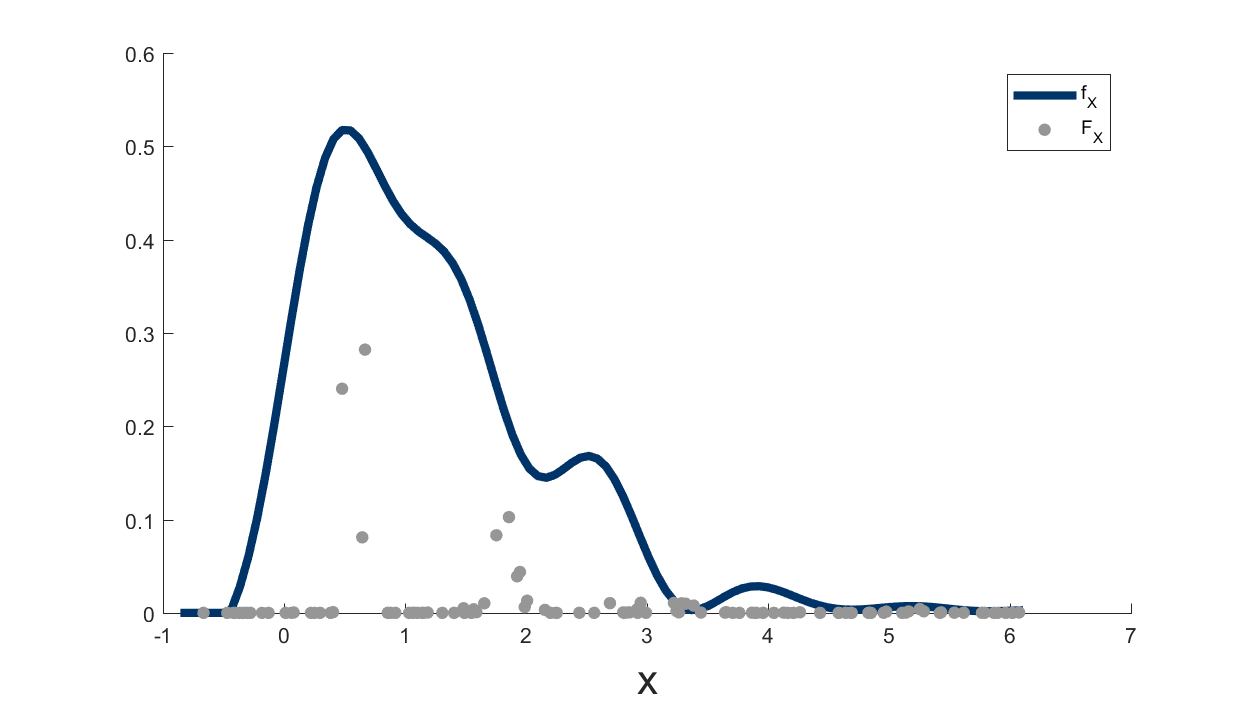
\includegraphics[width = \textwidth]{Figures/Deconvolution/fixed_masses_example.png}
		\caption{A typical deconvolution following the method of Delaigle and Hall \cite{Delaigle2016-la} with the continuous estimator $\hat{f}_X$.}
		\label{fig:fixed masses example alone}
	\end{figure}

	We wish to remark here that the conversion from the discrete $F_{\vect{\theta}, \vect{p}}$ to the continuous $\hat{f}_X$ has no effect on the phenomenon of interest in this chapter. We are mainly interested in the probability masses of the discrete distribution $F_{\vect{\theta}, \vect{p}}$. However, because we wish to include $\hat{f}_X(x)$ in our plots, we have included this section for completeness.

	




	% From here to the end of Section \ref{ssec:KernelSmoothing} is a summary of \cite{Delaigle2016-la}.
	% We want to find the distribution of a random variable $X$ but only measure 
	% $$W = X + U$$
	% where $U$ is symmetric (and hence $\phi_U(t)$ is real-valued and even). We also additionally require that $\phi_U(t) \geq 0$. We write
	% $$\rho_X = \frac{\phi_X}{|\phi_X|}$$
	% for the phase function of $X$. Then 
	% \begin{align*}
	% \phi_W &= \phi_X \phi_U	&&\text{as $X$ and $U$ are independent,}\\
	% \frac{\phi_W}{|\phi_W|} &= \frac{\phi_X}{|\phi_X|}\frac{\phi_U}{|\phi_U|},\\
	% \rho_W &= \rho_X	&&\text{as $\phi_U$ is real and non-negative.}
	% \end{align*}

	% Given a probability distribution, there are an infinite number of other distributions that have the same phase function. We make the choice that out of all the distributions with phase function $\rho_W$, we choose the one that has smallest variance. Hence, we want to find a distribution $F_Y$ that minimizes $\var(Y)$ such that
	% $$\rho_Y = \rho_W.$$

	% \subsection{Optimization problem}
	% 	\label{ssec:optimizationproblem}
	% 	Ideally, we would like to minimize the variance of $Y$ under the constraint that $\rho_Y = \rho_W$. However, we can't do this since we only estimate $\rho_W(t)$ from a random sample of size $n$ and this estimate is bad for large $|t|$. So we instead choose a $Y_0$ to minimize 
	% 	\begin{equation}
	% 	T(Y) = \int_{-\infty}^{\infty} \Big| \hat{\phi}_W(t) - |\hat{\phi}_W(t)| \rho_Y(t) \Big|^2 w(t) \intd t
	% 	\end{equation}\label{eq:T(Y)}
	% 	where $w(t)$ is some suitably chosen weight function and $\hat{\phi}_W(t)$ is our empirical estimate for $\phi_W(t)$. We then search for $Y$ which minimizes $\var(Y)$ subject to $T(Y) \leq T(Y_0)$.

	% 	We restrict our search to $Y$ discrete with point masses $p_j$ at locations $x_j$ for $j = 1,2,\dots,m$. We place our $x_j$ uniformly at random along the interval $[\min W, \max W]$ and choose the $p_j$ to solve the optimization problem described above. Numerical investigations indicate that $m = 5 \sqrt{n}$ is a reasonable choice.

	% \subsection{Kernel Smoothing}
	% 	\label{ssec:KernelSmoothing}
	% 	Once we have our discrete distribution $Y$ we can create a continuous density approximation using
	% 	\begin{equation}
	% 	\hat{f}_Y(x) = \frac{1}{2\pi} \int e^{-itx} \phi_Y(t) \phi_K(ht)  \intd t
	% 	\label{eq:f_Y(x)integral}
	% 	\end{equation}
	% 	where $K$ is some kernel with bandwidth $h$. This is exactly equivalent to
	% 	\begin{equation}
	% 	\hat{f}_Y(x) = \sum_{j=1}^m p_j K_h(x - x_j).
	% 	\label{eq:f_Y(x)sum}
	% 	\end{equation}

	% 	However, we can get a better result by using \eqref{eq:f_Y(x)integral} and replacing $\phi_Y(t)$ with an appropriate ridge function for $t \geq t^*$.
		%Ridging stuff
		%Choice of bandwidth
		%Integral considerations (stuff I did about how to integrate this thing)

% \FloatBarrier
\section{Empirical Results}
\label{sec:deconvolution empirical results}
% \section{Examples and Relation to Mixture Phenomenon}
	Following the methods outlined above, the authors noted that $F_{\vect{\theta}, \vect{p}}$ was usually supported on a small number of points. That is, only a few of the $p_j$ were non-zero. A typical example of this was given in Figures \ref{fig:fixed masses example no smoothing} and \ref{fig:fixed masses example alone}.

	% A theoretical justification for this behaviour is hard to obtain. We have made some observations which could be thought of as being in favour of this phenomenon, but mostly we are just pointing out similarities between this problem, and the maximum likelihood mixtures problem of the last chapter. These observations are left until Section \ref{sec:deconvolution observations and results}.

	A theoretical justification for this behaviour is hard to obtain. In Section \ref{sec:deconvolution observations and results} we make an observation about the problem which could be thought of as being in favour of this phenomenon, but for the most part, we have no rigourous explanation for why it occurs.

	In this section, we instead explore the phenomenon empirically, and suggest that we might benefit by allowing both the $\theta_j$ and $p_j$ to be the variables of our optimization, rather than fixing the $\theta_j$ as suggested in \cite{Delaigle2016-la}.

	We start by demonstrating the phenomenon using a variety of parameters and distributions. The base example (Figure \ref{fig:fixed masses example alone}) has the following setup:

	\begin{enumerate}
		\item The true distribution, $F_X$, is chi-squared with 3 degrees of freedom, rescaled to have variance $\sigma_X^2 = 1$.
		\label{enum: true F_X chi-squared}
		\item The error distribution, $F_U$, is normal.
		\label{enum: error F_U normal}
		\item The noise to signal ratio (NSR) is 1/5. That is, $\sigma_U^2 = \sigma_X^2 / 5$.
		\label{enum: NSR 1/5}
		\item We sample $n = 500$ points of $W = X+U$.
		\label{enum: n 500}
	\end{enumerate}

	As recommended in \cite{Delaigle2016-la}, we use $m = 5\sqrt{n}$ point masses in our approximating distribution $\hat{F}_X$. In Figures \ref{fig:fixed masses example Xgamma}, \ref{fig:fixed masses example Ucauchy}, \ref{fig:fixed masses example NSR1}, and \ref{fig:fixed masses example n10000} we change properties 1, 2, 3, and 4 respectively and plot the result. Of particular interest in each plot is $\hat{F}_X$ which we represent by placing a grey point at each probability mass. In each of these figures, as well as in the base example in Figure \ref{fig:fixed masses example alone}, we observe that the majority of the probability masses of $\hat{F}_X$ take values very close to, or equal to zero.

	% [MORE EXTENSIVE EXPLANATION OF WHAT'S GOING ON IN FIGURES???]

	% \begin{figure}
	% 	\centering
	% 	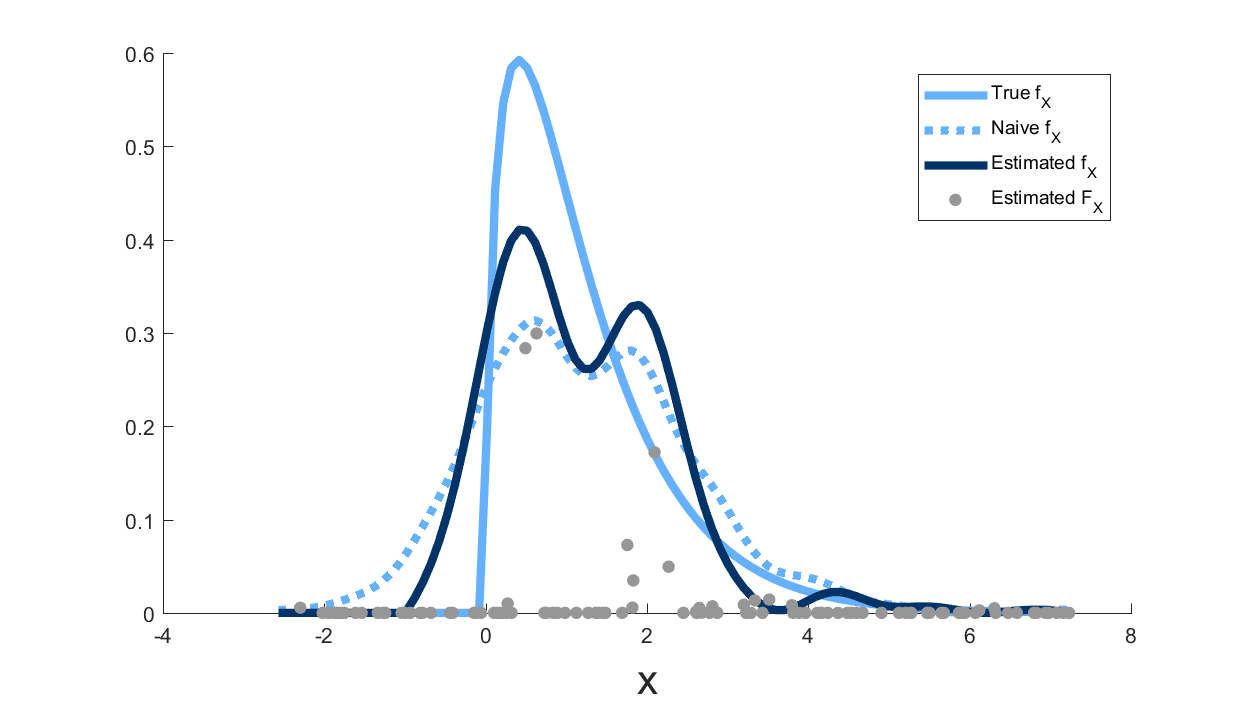
\includegraphics[width = \textwidth]{Figures/Deconvolution/fixed_masses_example_NSR1.png}
	% 	\caption{Blah}
	% 	\label{fig:fixed masses example NSR1}
	% \end{figure}

% [REGENERATE THESE FIGURE USING DESKTOP]
\begin{figure}
	\begin{subfigure}[b]{0.49\textwidth}
		\centering
		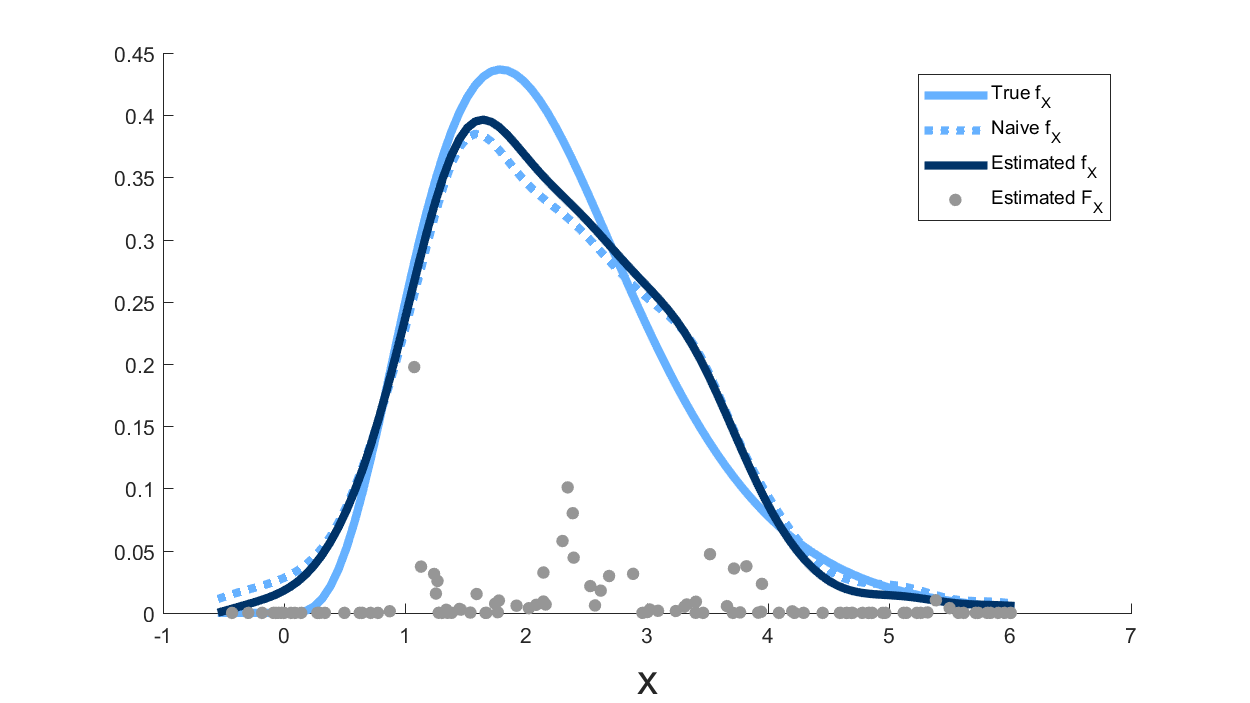
\includegraphics[width = \textwidth]{Figures/Deconvolution/fixed_masses_example_Xgamma.png}
		\caption{Using a Gamma(5,2) true distribution}
		\label{fig:fixed masses example Xgamma}
	\end{subfigure}
	\hfill
	\begin{subfigure}[b]{0.49\textwidth}
		\centering
		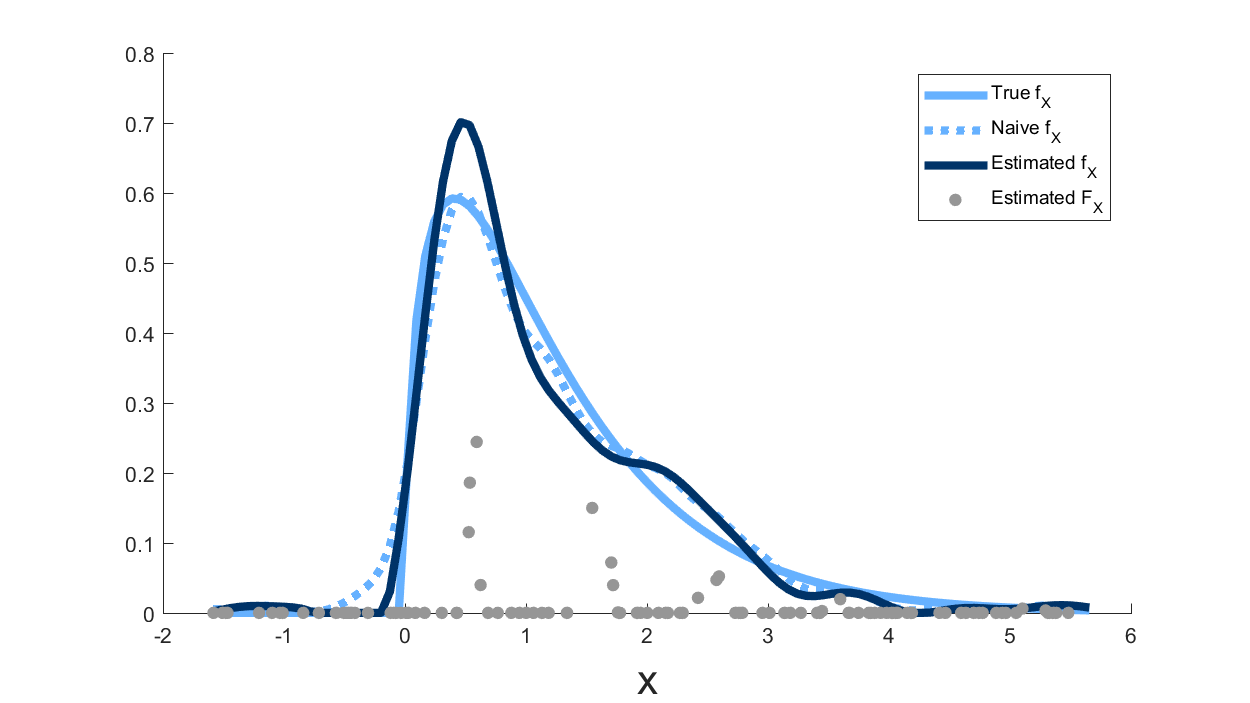
\includegraphics[width = \textwidth]{Figures/Deconvolution/fixed_masses_example_Ucauchy.png}
		\caption{Using a Cauchy error distribution}
		\label{fig:fixed masses example Ucauchy}
	\end{subfigure}
	\begin{subfigure}[b]{0.49\textwidth}
		\centering
		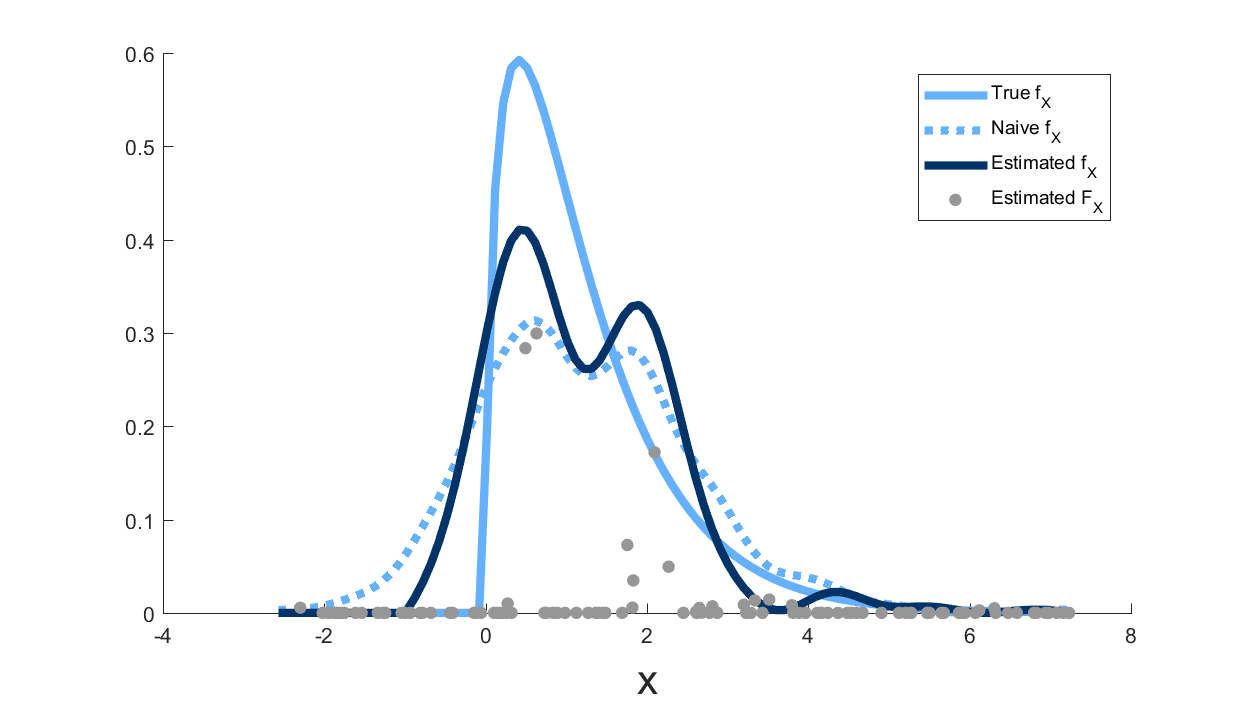
\includegraphics[width = \textwidth]{Figures/Deconvolution/fixed_masses_example_NSR1.png}
		\caption{Using a NSR of 1}
		\label{fig:fixed masses example NSR1}
	\end{subfigure}
	\hfill
	\begin{subfigure}[b]{0.49\textwidth}
		\centering
		% 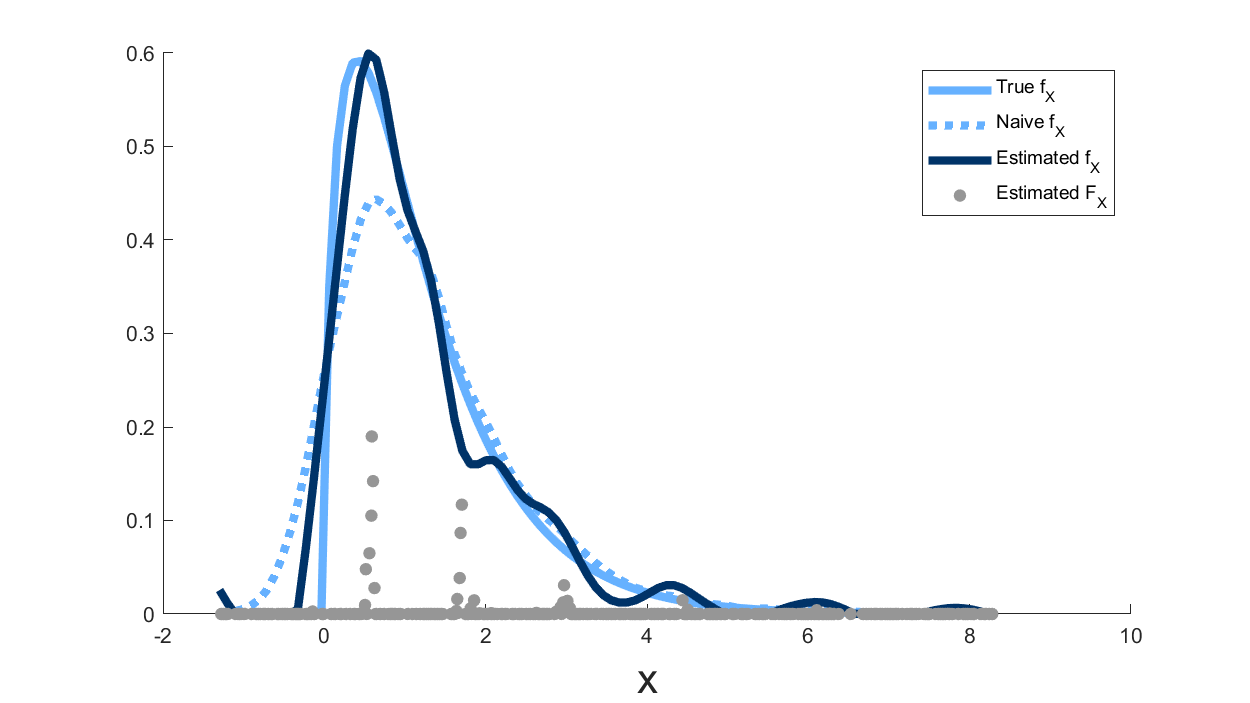
\includegraphics[width = \textwidth]{Figures/Deconvolution/fixed_masses_example_n10000.png}
		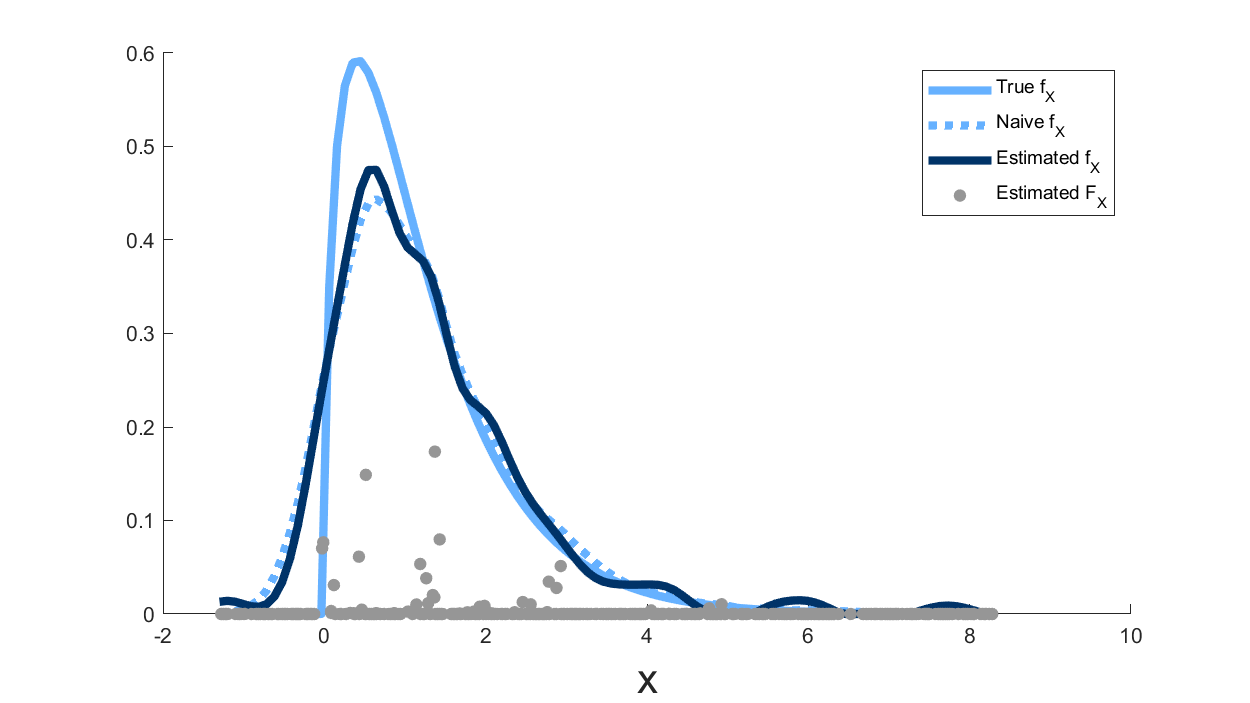
\includegraphics[width = \textwidth]{Figures/Deconvolution/fixed_masses_example_n10000_updated.png}
		\caption{Using $n = 10000$ points}
		\label{fig:fixed masses example n10000}
	\end{subfigure}
	\caption{Four variations on the base example in Figure \ref{fig:fixed masses example alone}.}
	\label{fig:comparison different fixed masses examples}
\end{figure}

Given that most of the probability masses of $\hat{F}_X$ do not contribute to the final density, we might hope to reduce the complexity of our optimization problem by using a more appropriate number of masses. Of course, we do not know a priori where these masses should be located along the x axis, and so should make their locations variables in our optimization. While this essentially doubles the dimension of our optimization, we suspect that we will need fewer than half the original number of points and so do not expect a computational slow down. In the figures above, we observe that roughly 10 to 20 points out of $m = 112$ or $m = 500$ masses have weights that are visibly greater than 0. Furthermore, it is feasible that two points located close to each other might coalesce into a single point in such a way as to improve the objective if their locations are allowed to vary. This encourages us to proceed using roughly 10 to 20 probability masses with variable weights and locations for $\hat{F}_X$.

\begin{figure}
	\centering
	\begin{subfigure}[b]{0.49\textwidth}
		\centering
		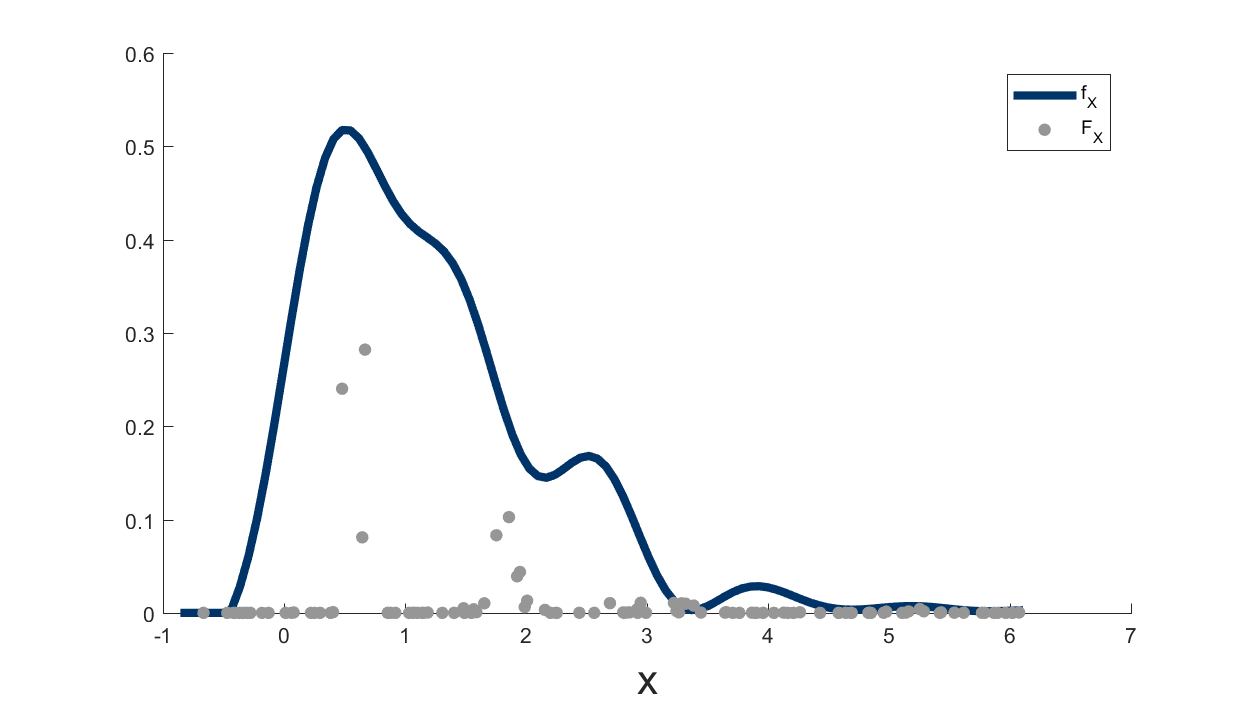
\includegraphics[width = \textwidth]{Figures/Deconvolution/fixed_masses_example.png}
		\begin{tabular}{r l}
			$OBJ_1$ & 0.2284\\
			$\var \hat{F}_X$ & 0.8613\\
			$T(\hat{F}_X)$ & 3.8697e-07\\
			$P_1$ & 4.5679e-04\\
			$P_2$ & 0\\
			$t$ & 195s
		\end{tabular}
		\caption{112 fixed masses}
		\label{fig:fixed masses example}
	\end{subfigure}
	\hfill
	\begin{subfigure}[b]{0.49\textwidth}
		\centering
		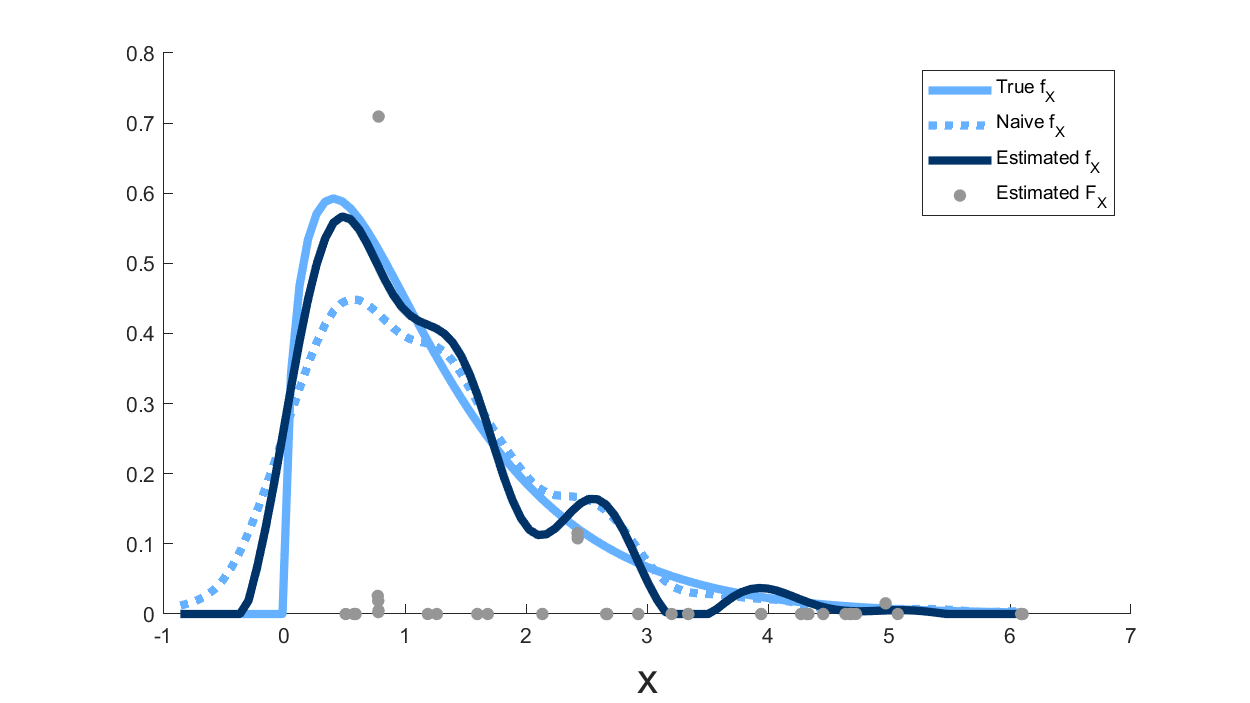
\includegraphics[width = \textwidth]{Figures/Deconvolution/moving_masses_m40_example.png}
		\begin{tabular}{r l}
			$OBJ_1$ & 54.3622\\
			$\var \hat{F}_X$ & 0.6554\\
			$T(\hat{F}_X)$ & 1.7882e-06\\
			$P_1$ & 0.1087\\
			$P_2$ & 0\\
			$t$ & 76s
		\end{tabular}
		\caption{40 moving masses}
		\label{fig:moving masses m40 example}
	\end{subfigure}
	\begin{subfigure}[b]{0.49\textwidth}
		\centering
		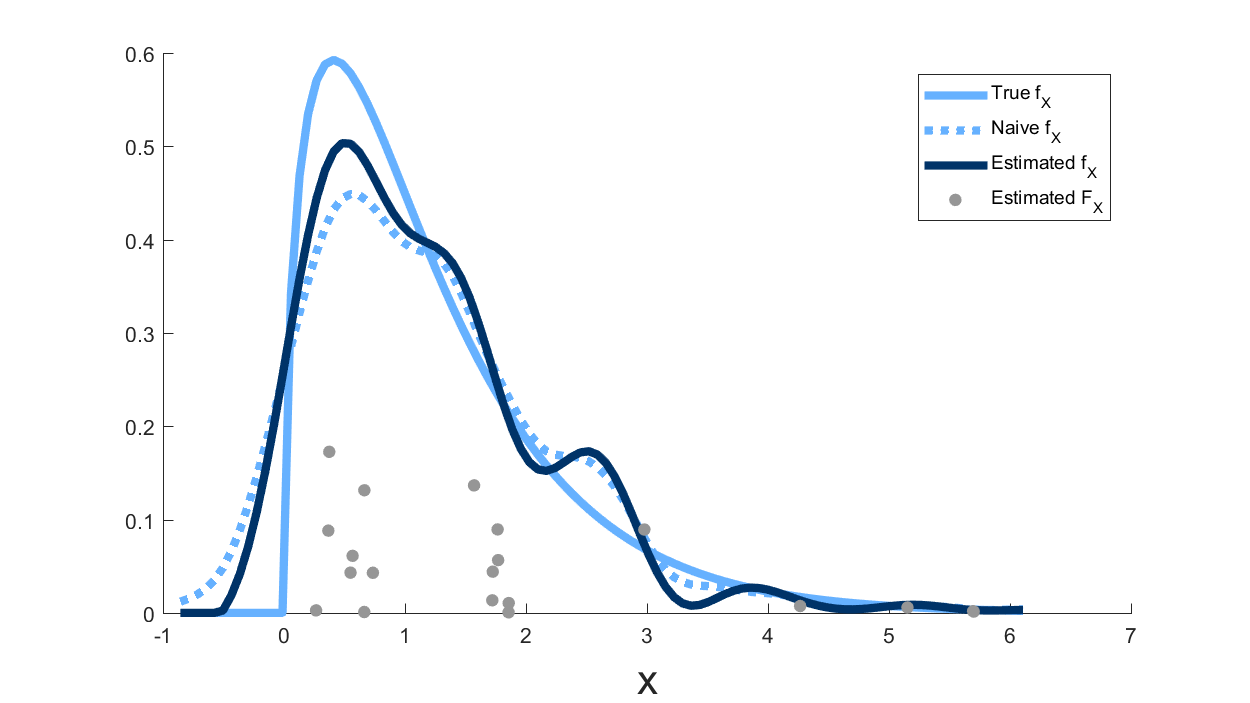
\includegraphics[width = \textwidth]{Figures/Deconvolution/moving_masses_m20_example.png}
		\begin{tabular}{r l}
			$OBJ_1$ & 0.0396\\
			$\var \hat{F}_X$ & 0.8042\\
			$T(\hat{F}_X)$ & 4.4981e-07\\
			$P_1$ & 7.9209e-05\\
			$P_2$ & 0\\
			$t$ & 37s
		\end{tabular}
		\caption{20 moving masses}
		\label{fig:moving masses m20 example}
	\end{subfigure}
	\hfill
	\begin{subfigure}[b]{0.49\textwidth}
		\centering
		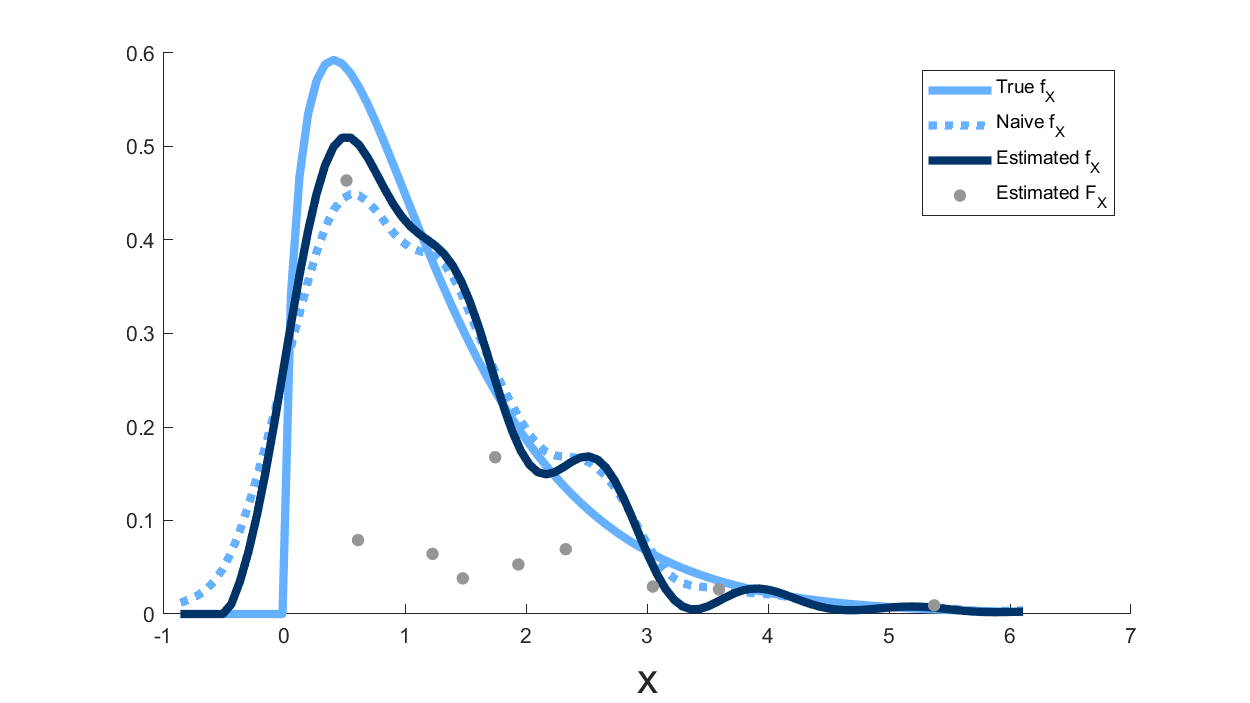
\includegraphics[width = \textwidth]{Figures/Deconvolution/moving_masses_m10_example.png}
		\begin{tabular}{r l}
			$OBJ_1$ & 0.1374\\
			$\var \hat{F}_X$ & 0.8269\\
			$T(\hat{F}_X)$ & 4.2464e-07\\
			$P_1$ & 2.7478e-04\\
			$P_2$ & 0\\
			$t$ & 15s
		\end{tabular}
		\caption{10 moving masses}
		\label{fig:moving masses m10 example}
	\end{subfigure}
	\begin{subfigure}[b]{0.49\textwidth}
		\centering
		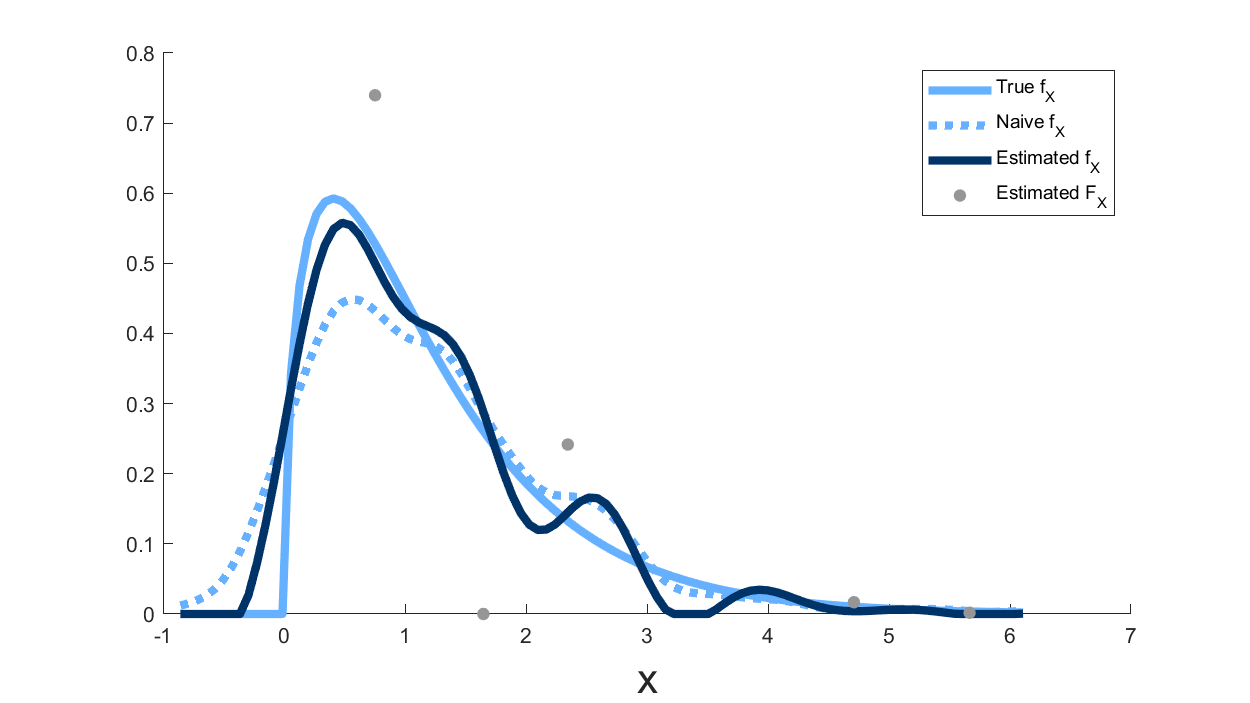
\includegraphics[width = \textwidth]{Figures/Deconvolution/moving_masses_m5_example.png}
		\begin{tabular}{r l}
			$OBJ_1$ & 0.3905\\
			$\var \hat{F}_X$ & 0.8888\\
			$T(\hat{F}_X)$ & 3.6213e-07\\
			$P_1$ & 7.8093e-04\\
			$P_2$ & 0\\
			$t$ & 4s
		\end{tabular}
		\caption{5 moving masses}
		\label{fig:moving masses m5 example}
	\end{subfigure}
	\hfill
	\begin{subfigure}[b]{0.49\textwidth}
		\centering
		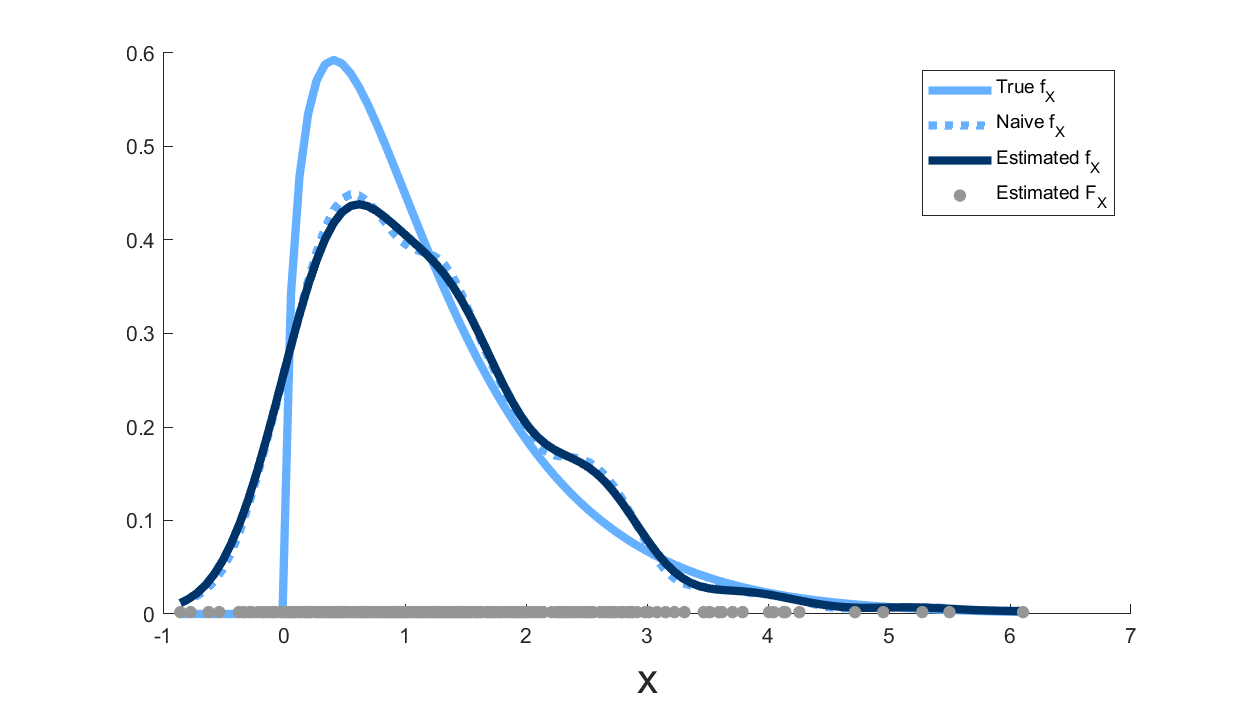
\includegraphics[width = \textwidth]{Figures/Deconvolution/emp_masses_example.png}
		\begin{tabular}{r l}
			$OBJ_1$ & 2.7811e-07\\
			$\var \hat{F}_X$ & 1.0350\\
			$T(\hat{F}_X)$ & 2.7810e-07\\
			$P_1$ & 1.0079e-14\\
			$P_2$ & 1.7097e-14\\
			$t$ & NA
		\end{tabular}
		\caption{The empirical distribution of W}
		\label{fig:emp masses example}
	\end{subfigure}
	
	\caption{Comparison of results between fixed and variable probability mass locations.}
	\label{fig:compare fixed moving masses}
\end{figure}

We start with Figure \ref{fig:compare fixed moving masses} in which we compare the result we obtain using the fixed but random location method of Delaigle and Hall \cite{Delaigle2016-la}, and the results we obtain when we allow the location of the probability masses in $F_{\vect{\theta}, \vect{p}}$ to vary. As well as plotting $\hat{F}_X$ and $\hat{f}_X$, we also provide a table with the various objective values obtained in the final result, as well as the time taken to run the code on a i5-4670K CPU running at 4.3 GHz, running MATLAB R2018a. For comparison, we also give the various objective values obtained by using the empirical distribution of $W$ as $\hat{F}_X$. The values $T$, $P_1$, $P_2$ are as defined in Section \ref{sec:deconvolution estimator}, we use $OBJ1$ to denote the objective of our first minimization, $T(F) + \lambda_1 P_1(F) + \lambda_2 P_2(F)$, and $\var$ to denote the variance of $\hat{F}_X$ (our second objective).

For this particular example, we note that we need only 10 masses (Figure \ref{fig:moving masses m10 example}) to obtain smaller values for both of our objectives when compared to the original fixed masses, and that this results in a significant speed up, as expected. We get even further improvement going from 10 to 20 masses (Figure \ref{fig:moving masses m20 example}). However, when we use 40 masses (Figure \ref{fig:moving masses m40 example}), we note that $OBJ_1$ is significantly larger than in any of the cases where we use fewer masses, and that $\var\hat{F}_X$ is smaller than in any other case. One potential explanation here is that the parameter space becomes too complex for our optimization routine to find good solutions if we allow too many moving masses and so $OBJ_1$ is much larger than the global minimum. This means that when we come to our second objective of minimizing $\var \hat{F}_X$, the constraints $T(F) \leq T_\mathrm{min}$, $P_1(F) \leq P_1^\mathrm{min}$, and $P_2(F) \leq P_2^\mathrm{min}$ are lax, and so we have more room to search for feasible distributions with small variance.

It also appears as if the 40 mass case is a closer fit for the true curve than any of the other estimates, despite achieving worse results in the first objective. Although this is purely conjecture, we suggest that this could be because the constraints $T(F) \leq T_\mathrm{min}$, $P_1(F) \leq P_1^\mathrm{min}$, and $P_2(F) \leq P_2^\mathrm{min}$ are often too strict to achieve the variance we desire in the second optimization. The first optimization found a solution which just happened to be far enough away from the global minimum to allow for enough freedom in minimizing the variance that we obtained a result that achieved closer to the true variance. One could try using as constraints, $T(F) \leq (1 + \delta) T_\mathrm{min}$, $P_1(F) \leq (1 + \delta) P_1^\mathrm{min}$, and $P_2(F) \leq (1 + \delta) P_2^\mathrm{min}$, to allow for this behaviour when the first minimization attains a result closer to the global optimum, but we cannot see any obvious way to determine good values for $\delta$.

The results in Figure \ref{fig:compare fixed moving masses} are encouraging, and in our experience are consistent in a wide variety of scenarios. We present some more examples in Figure \ref{fig:more deconvolution examples}. 
In this figure we compare the fixed but random location method with the varying location method for three different scenarios. A discrete true distribution with normal errors and $n = 5000$ observations (Figures \ref{fig:moving masses discrete} and \ref{fig:fixed masses discrete}), a Gumbel true distribution with Laplace errors and $n = 500$ observations (Figures \ref{fig:moving masses gumbel lap} and \ref{fig:fixed masses gumbel lap}), and a Gamma with shape 5 and rate 2 true distribution with discrete errors and $n = 100$ observations (Figures \ref{fig:moving masses gamma discrete} and \ref{fig:fixed masses gamma discrete}). For the varying location method we use $m = 20$ masses and for the fixed but random location method we use $m = 5\sqrt{n}$ masses. In each scenario we observe that the varying location method is much faster, and in two of the three scenarios produces better objective values. In the scenario where the varying location method did not produce as good results (Figures \ref{fig:moving masses gumbel lap} and \ref{fig:fixed masses gumbel lap}), the fixed location method only assigned approximately 12 or 13 points weights that were noticeably larger than zero and the varying location method made several point masses redundant. This suggests that the slightly worse result of the varying location method is not due to using too few points.

% [GIVE AN EXPLANATION OF WHAT IS HAPPENING]

Of course, it is possible that there is a wide class of deconvolution problems in which a large number of point masses are required to achieve a good solution, and that we have just happened to avoid examples of these. However, we do not think that this is the case, and even if it is, we do not think that this is a large concern. One can simply repeat the deconvolution with an increasing number of point masses in $\hat{F}_X$ until it does not result in an improvement in our objectives.

\begin{figure}
	\centering
	\begin{subfigure}[b]{0.38\textwidth}
		\centering
		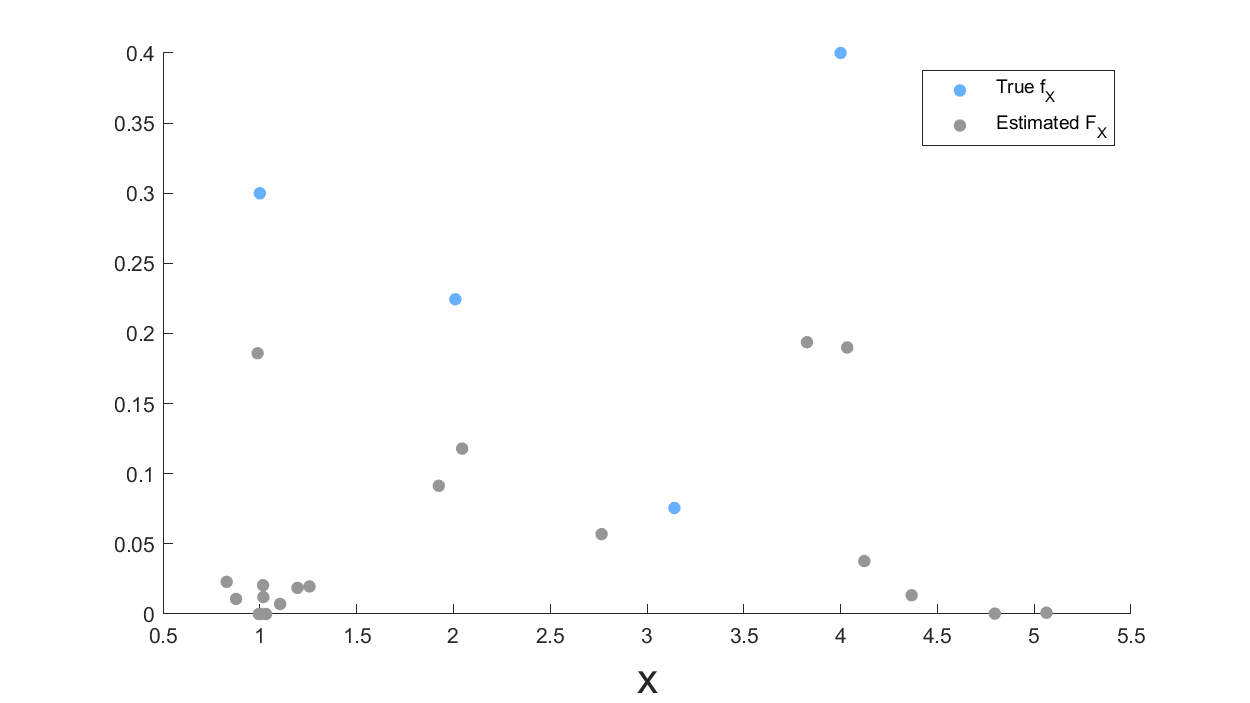
\includegraphics[width = \textwidth]{Figures/Deconvolution/moving_masses_discrete_n5000_example.png}
		\begin{tabular}{r l}
			$OBJ_1$ & 0.8786\\
			$\var \hat{F}_X$ & 1.6542\\
			$T(\hat{F}_X)$ & 1.1094e-08\\
			$P_1$ & 0.0018\\
			$P_2$ & 0\\
			$t$ & 62s
		\end{tabular}
		\caption{True distribution discrete (represented by blue points) with normal errors, $n = 5000$, moving masses.}
		\label{fig:moving masses discrete}
	\end{subfigure}
	\hfill
	\begin{subfigure}[b]{0.38\textwidth}
		\centering
		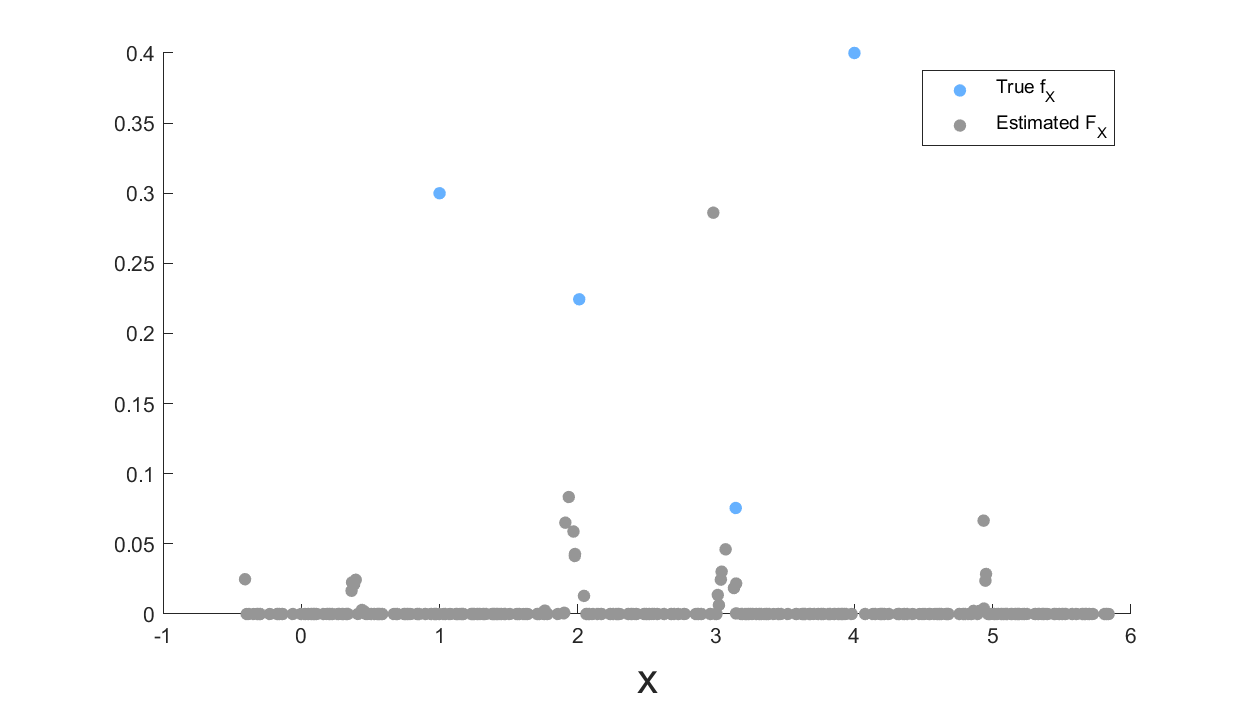
\includegraphics[width = \textwidth]{Figures/Deconvolution/fixed_masses_discrete_n5000_example.png}
		\begin{tabular}{r l}
			$OBJ_1$ & 106.6533\\
			$\var \hat{F}_X$ & 1.5731\\
			$T(\hat{F}_X)$ & 0.0192\\
			$P_1$ & 0.2133\\
			$P_2$ & 0\\
			$t$ & 1354s
		\end{tabular}
		\caption{True distribution discrete (represented by blue points) with normal errors, $n = 5000$, fixed masses.}
		\label{fig:fixed masses discrete}
	\end{subfigure}
	\begin{subfigure}[b]{0.38\textwidth}
		\centering
		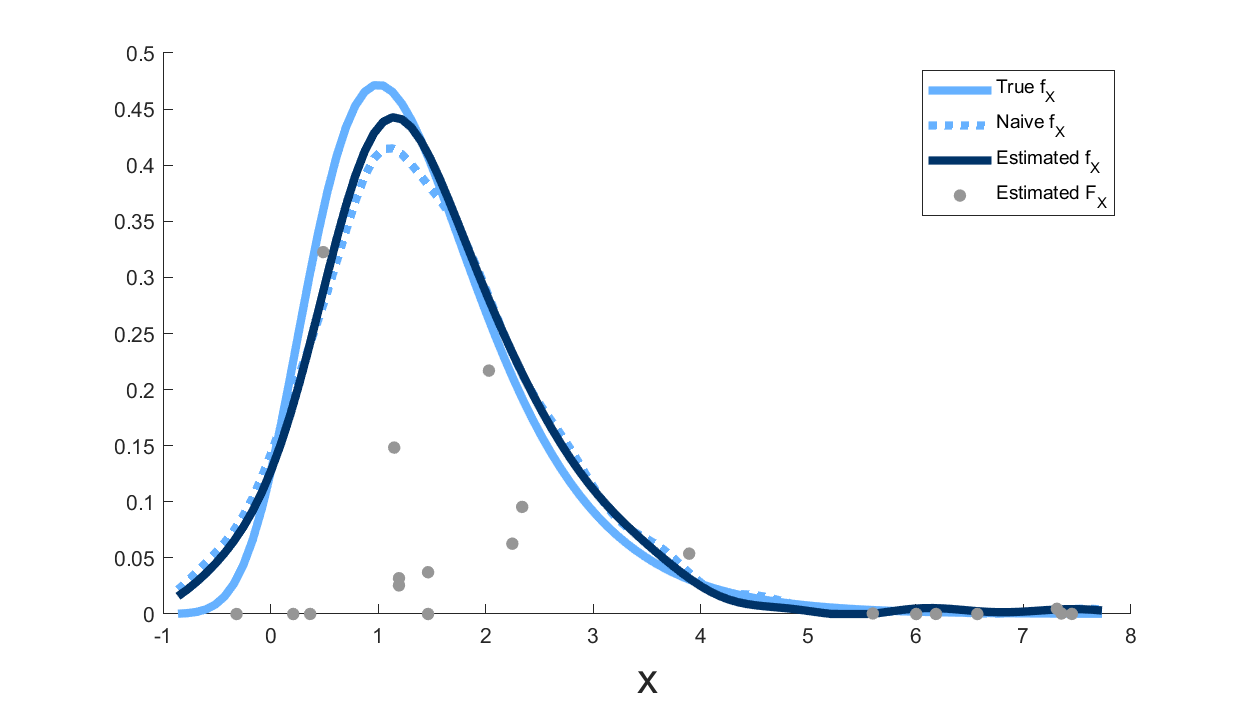
\includegraphics[width = \textwidth]{Figures/Deconvolution/moving_masses_gumbel_lap_example.png}
		\begin{tabular}{r l}
			$OBJ_1$ & 0.3742\\
			$\var \hat{F}_X$ & 1.0063\\
			$T(\hat{F}_X)$ & 3.5329e-07\\
			$P_1$ & 7.4839e-04\\
			$P_2$ & 0\\
			$t$ & 64s
		\end{tabular}
		\caption{True distribution Gumbel with Laplace errors, $n = 500$, moving masses.}
		\label{fig:moving masses gumbel lap}
	\end{subfigure}
	\hfill
	\begin{subfigure}[b]{0.38\textwidth}
		\centering
		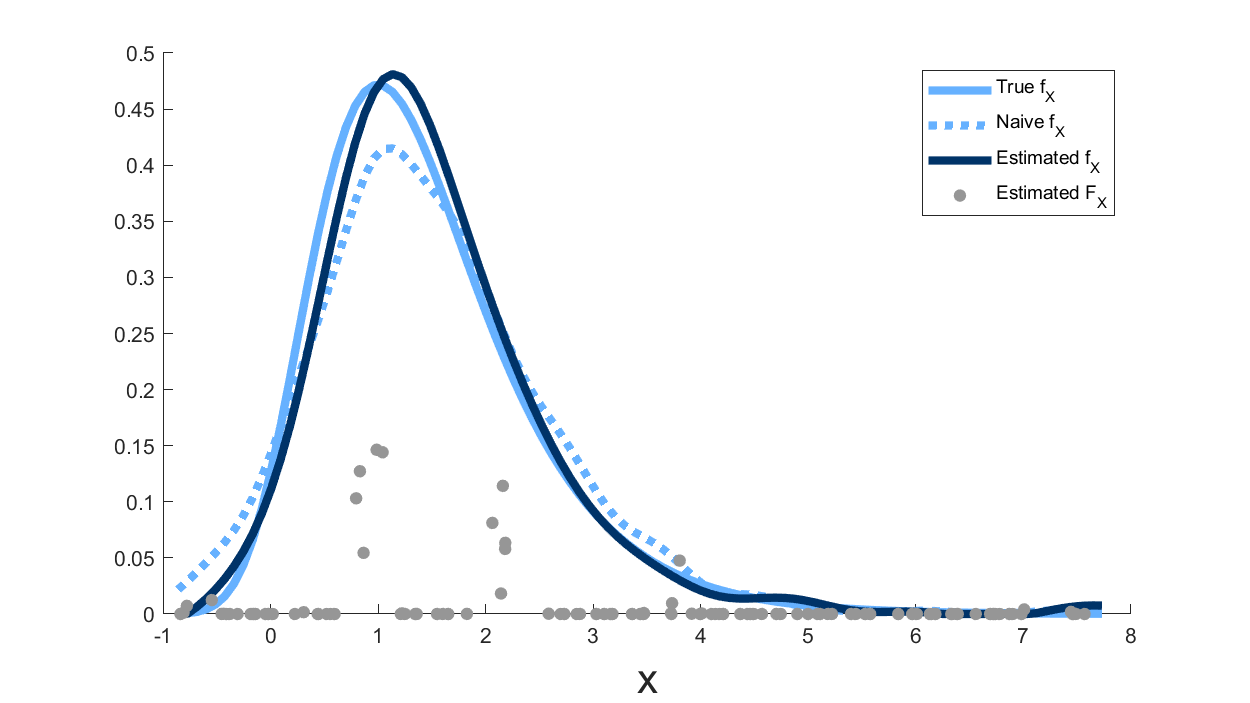
\includegraphics[width = \textwidth]{Figures/Deconvolution/fixed_masses_gumbel_lap_example.png}
		\begin{tabular}{r l}
			$OBJ_1$ & 0.2603\\
			$\var \hat{F}_X$ & 0.9413\\
			$T(\hat{F}_X)$ & 4.9281e-07\\
			$P_1$ & 5.2056e-04\\
			$P_2$ & 0\\
			$t$ & 195s
		\end{tabular}
		\caption{True distribution Gumbel with Laplace errors, $n = 500$, fixed masses.}
		\label{fig:fixed masses gumbel lap}
	\end{subfigure}
	\begin{subfigure}[b]{0.38\textwidth}
		\centering
		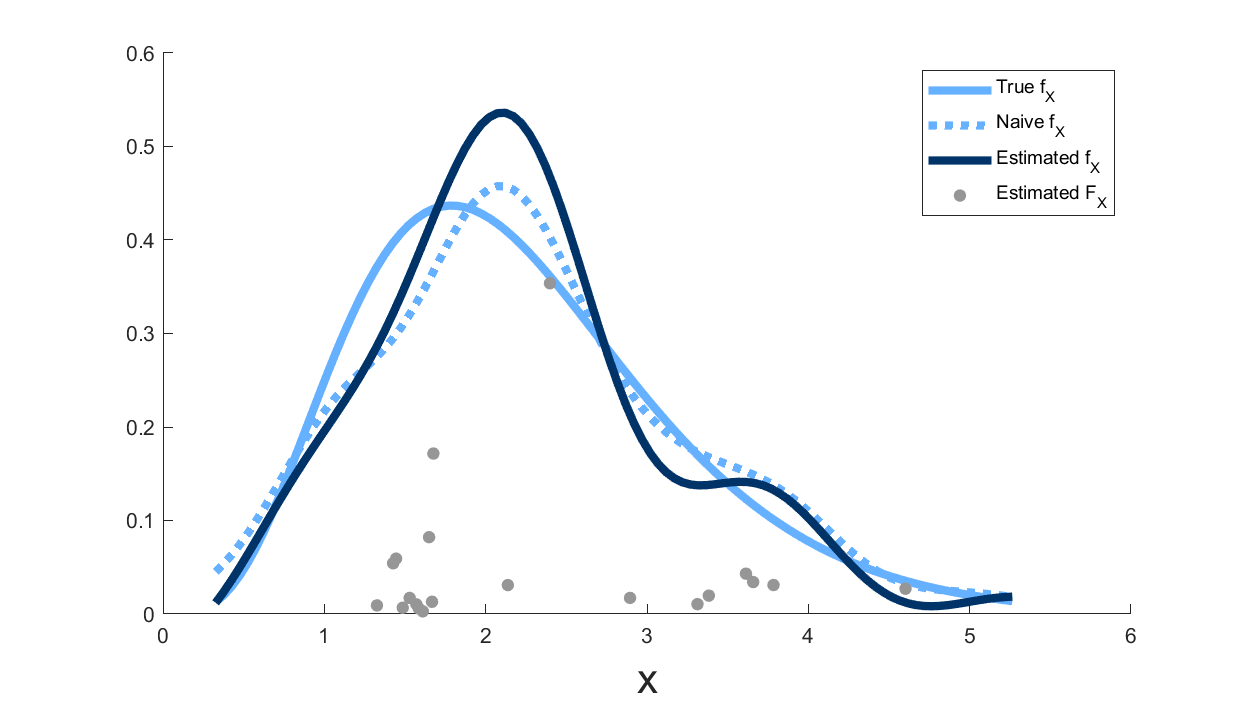
\includegraphics[width = \textwidth]{Figures/Deconvolution/moving_masses_gamma_discrete_n100_example.png}
		\begin{tabular}{r l}
			$OBJ_1$ & 0.1506\\
			$\var \hat{F}_X$ & 0.6176\\
			$T(\hat{F}_X)$ & 1.2286e-05\\
			$P_1$ & 3.0108e-04\\
			$P_2$ & 0\\
			$t$ & 47s
		\end{tabular}
		\caption{True distribution Gamma(5,2), with errors discrete (-1,0,1) with probabilities (0.2,0.6,0.2), $n = 100$, moving masses.}
		\label{fig:moving masses gamma discrete}
	\end{subfigure}
	\hfill
	\begin{subfigure}[b]{0.38\textwidth}
		\centering
		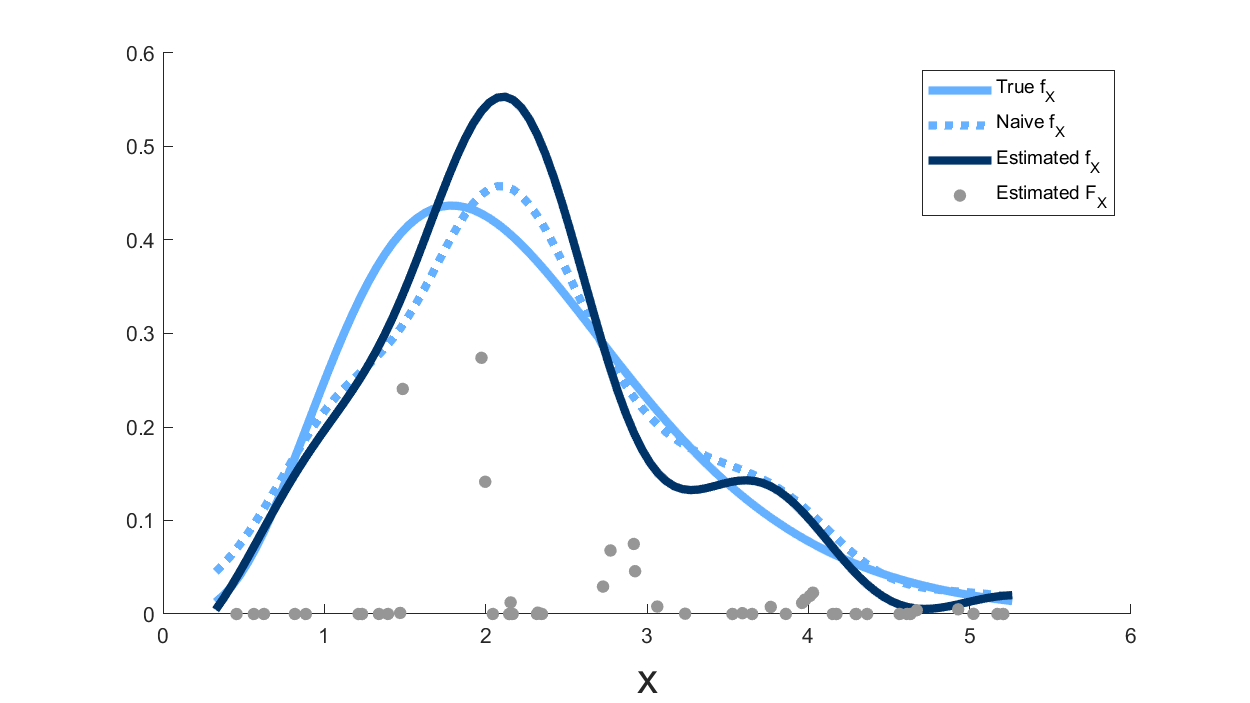
\includegraphics[width = \textwidth]{Figures/Deconvolution/fixed_masses_gamma_discrete_n100_example.png}
		\begin{tabular}{r l}
			$OBJ_1$ & 0.1681\\
			$\var \hat{F}_X$ & 0.5953\\
			$T(\hat{F}_X)$ & 1.2921e-05\\
			$P_1$ & 3.3615e-04\\
			$P_2$ & 0\\
			$t$ & 62s
		\end{tabular}
		\caption{True distribution Gamma(5,2), with errors discrete (-1,0,1) with probabilities (0.2,0.6,0.2), $n = 100$, fixed masses.}
		\label{fig:fixed masses gamma discrete}
	\end{subfigure}
	\caption{Three more comparisons between moving masses and fixed masses.}
	\label{fig:more deconvolution examples}
	\end{figure}

\subsection{R Package}
Given all the discussion above, we see no reason not to use masses with variable locations. We have used this new method in the R \cite{R_Core_Team2018-bs} Package `deconvolve' \cite{Delaigle2019-hj}. This package is a collection of tools for performing non-parametric deconvolution on measurement error problems. It contains functions for finding bandwidths, deconvolved densities, and non-parametric regression estimates. The methods discussed in this chapter for when the error distribution is unknown form just one part of the package. We give a brief overview of the performance of our implementation of it in R.

\begin{figure}
	\centering
	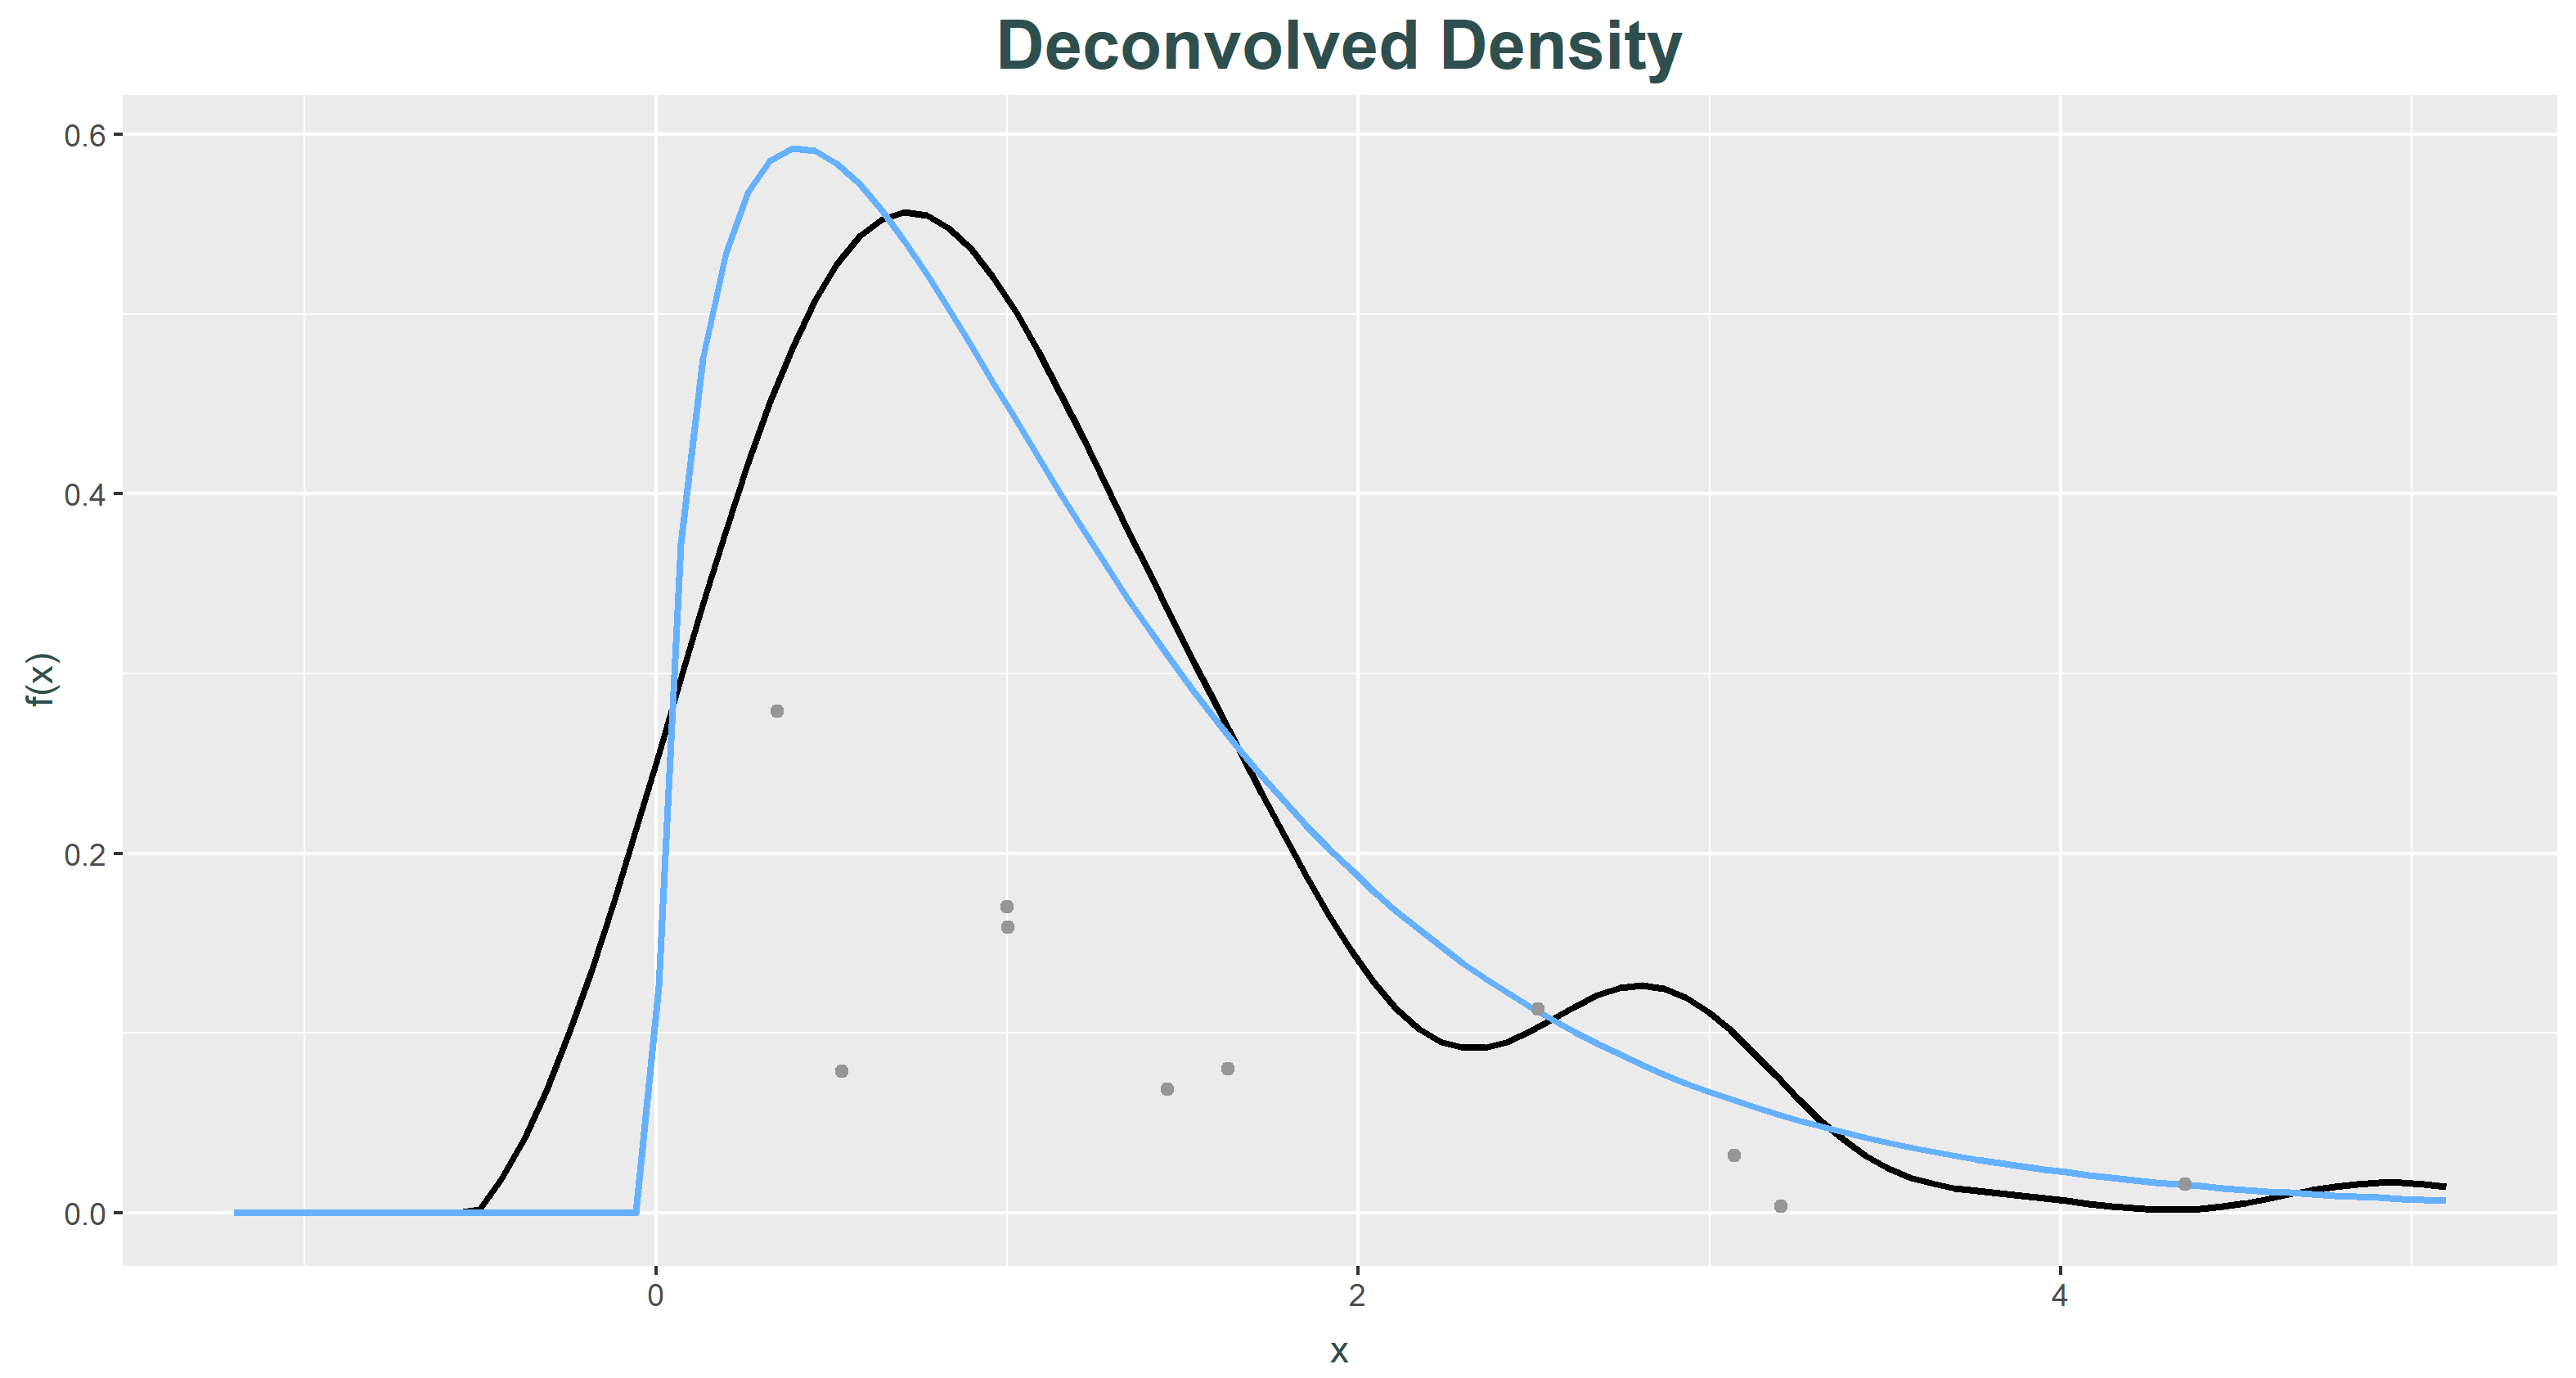
\includegraphics[width = \textwidth]{Figures/Deconvolution/R_example.png}
	\begin{tabular}{r l}
			$OBJ_1$ & 2.277\\
			$\var \hat{F}_X$ & 0.8684\\
			$T(\hat{F}_X)$ & 1.1672e-06\\
			$P_1$ & 4.554e-03\\
			$P_2$ & 0\\
			$t$ & 50s
		\end{tabular}
	\caption{The output of the `deconvolve' package with data as in Figure \ref{fig:fixed masses example alone} and using $m=20$ moving masses.}
	\label{fig:R example}
\end{figure}

In Figure \ref{fig:R example}, we show the output of our package when the contaminated data is identical to that used in producing Figure \ref{fig:fixed masses example alone}. As in Figure \ref{fig:compare fixed moving masses}, we provide the values obtained of each of our objectives, as well as the time taken to run.

To perform the two non-linear optimizations we use the package Nlcoptim \cite{Chen2017-mn}. In the example in Figure \ref{fig:R example}, we used 20 moving masses in our estimate $\hat{F}_X$. This make it directly comparable to \ref{fig:moving masses m20 example}, since we are using identical data and parameters. While the objective values obtained are worse than those in the equivalent MATLAB implementation, the resulting density is still reasonable and we still benefit from a significant speed up over the original fixed mass implementation. In practice, we found this to be fairly typical of our implementation in `deconvolve'. 

We are unsure as to why our implementation in R tends to produce worse objective values than our implementation in MATLAB. We suspect that the optimization routines used in MATLAB's \emph{fmincon} function are more powerful than those used in the Nlcoptim package for R, but we do not know exactly what is going on. However, we are not particularly concerned about it since despite the difference in objective values, the estimated densities we obtain using R appear to be just as good as those we get in MATLAB. This could also be related to the discussion earlier in this section about Figure \ref{fig:moving masses m40 example} in which we pointed out that worse objective values in our first optimization can sometimes produce better looking densities.

% [WHY IS R WORSE?]

% [UP TO HERE]

% [R NOT AS GOOD RESULTS]

% [STILL FAST THOUGH]

% [PUT IN TIME COMPARISONS HERE]

% \begin{figure}
% 	\centering
% 	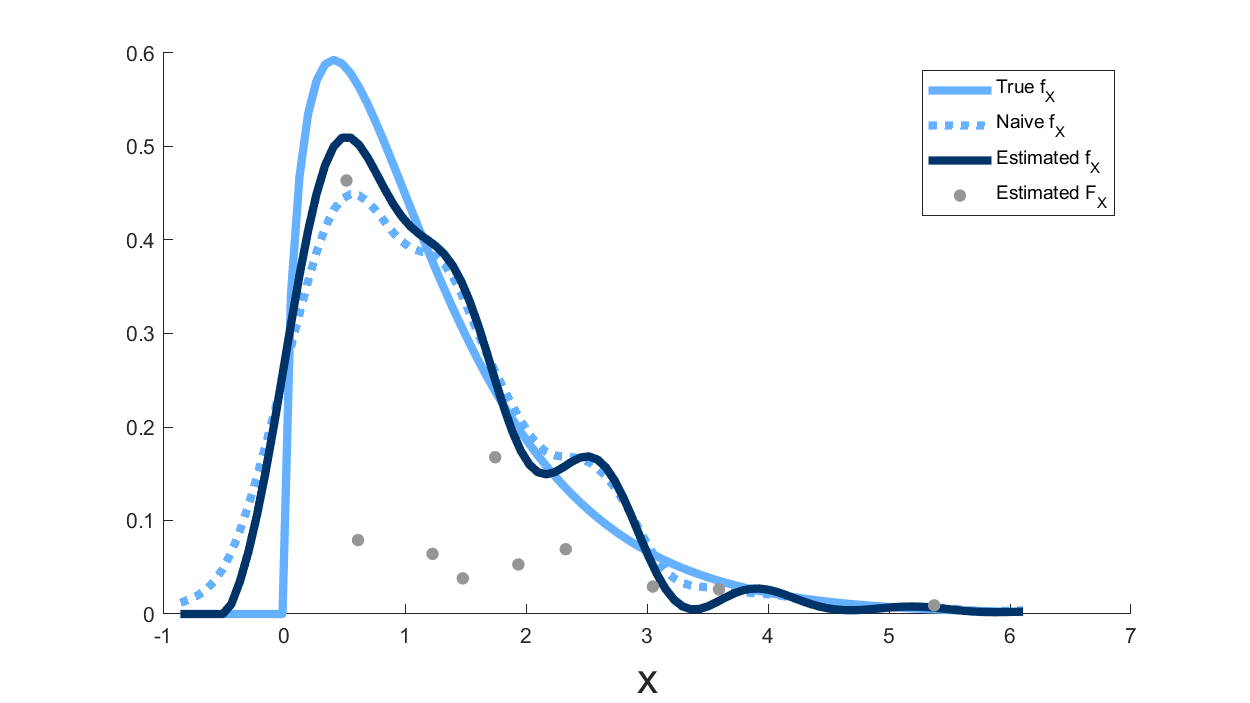
\includegraphics[width = \textwidth]{Figures/Deconvolution/moving_masses_m10_example.png}
% 	\begin{tabular}{r l}
% 		$\var \hat{F}_X$ & 0.9011\\
% 		$T(\hat{F}_X)$ & 3.5540e-07\\
% 		$P_1$ & 7.0136e-05\\
% 		$P2$ & 0\\
% 		$t$ & 492
% 	\end{tabular}
% 	\caption{blah}
% 	\label{fig:moving masses m10 example}
% \end{figure}



% \subsection{No penalties seems to make behaviour stronger}

% \subsection{Discrete X?}

	

\section{General observations and results}
\label{sec:deconvolution observations and results}

We end this chapter by making some comparisons between our deconvolution problem, and the maximum likelihood location mixture problem of Chapter \ref{Ch:Mixtures}.

% \subsection{Not the same}
In Chapter \ref{Ch:Mixtures}, we defined a quantity $K_\vect{x}$ \eqref{eq:K_x definition} which counted the number of components in the maximum likelihood mixture. One might think to define an analogous quantity here, $K_W$, which counts the number of point masses required to find the global optimum to our optimization problem. However, we do not think that this would be a very useful construct. Consider the empirical distribution of $W$, $\hat{F}_W$. We trivially have that $P_1(\hat{F}_W) = P_2(\hat{F}_W) = 0$ and that $T(\hat{F}_W)$ is very close to zero (it would be exactly zero if we replaced $|\hat{\psi}_W|^{1/2}$ with $|\hat{\phi}_W|$). We suspect that $OBJ_1$ will typically be much smaller for $\hat{F}_W$ than for distributions with fewer than $n$ points of support (see for example Figure \ref{fig:emp masses example}, and compare with the other figures in Figure \ref{fig:compare fixed moving masses}) and so we would have $K_W \geq n$. This is clearly much larger than the quantity we are interested in.

Another approach we used in Chapter \ref{Ch:Mixtures} was to explicitly write out our optimization problem in terms of the $\theta_j$s and $p_j$s (see Section \ref{sec:KKT conditions}). However, in the deconvolution setting, this becomes more complex. Even if we ignore our two penalties (and these might even simply be implementation details that are obscuring the basic problem), the problem becomes that of finding the $\vect{\theta}$ and $\vect{p}$ that minimize
\begin{equation}
	\var(F_{\vect{\theta}, \vect{p}}) = \left(\sum_{j =1}^m p_j \theta_j^2 \right) - \left(\sum_{j = 1}^m p_j \theta_j \right)^2
\end{equation}
subject to the constraints
\begin{align}
	&\theta_j -\theta_{j+1} \leq 0, &&j=1,\dots,m-1	\label{eq:decon constraint 1}\\
	&-p_j \leq 0, &&j=1,\dots,m	\label{eq:decon constraint 2} \\
	&\sum_{j=1}^m p_j = 1.
	\label{eq:decon constraint 3}
\end{align}
and
\begin{equation}
	\int_{-\infty}^\infty \left| \hat{\phi}_W(t) \left|\sum_{j = 1}^m p_j \exp(it\theta_j)\right| - \left|\hat{\psi}_W(t)\right|^{1/2} \left(\sum_{j = 1}^m p_j \exp(it\theta_j) \right)\right|^2 w_1(t) \intd t \leq T^\mathrm{min}.
\end{equation}
It is this last constraint which makes a similar analysis difficult. However, it is still worth noting that constraints \eqref{eq:decon constraint 1} to \eqref{eq:decon constraint 3} are shared with the maximum likelihood optimization problem (in both problems we are searching for a discrete probability distribution), and that perhaps these constraints contribute to the phenomenon of interest.
% \begin{equation}
% 	\sum_{j = 1}^m p_j \exp(it\theta_j)
% \end{equation}

% [NOT AS CLEAN AS MIXTURES, COULD POINT OUT BY WRITING PROBLEM WITH THETAS AND PS]

% \subsection{Simple observation}

We now make a simple observation about our deconvolution problem. We do not claim that it is new, but we think that it is still worth stating because it establishes another connection between our deconvolution problem, and the mixture problem of Chapter \ref{Ch:Mixtures}.

	% \subsection{Results concerning phase functions}
	\begin{theorem}
	\label{thm:equal phase functions convex set}
		Let $F_1$ and $F_2$ be two distributions with phase functions $\rho_1$ and $\rho_2$, and let
		\begin{align}
			F_Z &= (1 - \lambda) F_1 + \lambda F_2, && \lambda \in [0,1]
		\end{align}
		be a convex combination of these distributions. If $\rho_1 = \rho_2$, then 
		\begin{equation}
			\rho_Z = \rho_1 = \rho_2.
		\end{equation}
	\end{theorem}
	\begin{proof}
		Write $\phi_1$ and $\phi_2$ for the characteristic functions of $F_1$ and $F_2$. These are complex valued functions which we can write in the form
		\begin{align}
			\phi_1(t) &= r_1(t) \euler^{i\theta_1(t)},\\
			\phi_2(t) &= r_2(t) \euler^{i\theta_2(t)},
		\end{align}
		where $r_1(t), r_2(t)$ take values on $[0, 1]$ and where
		\begin{align}
			\rho_1(t) &= \euler^{i\theta_1(t)},\\
			\rho_2(t) &= \euler^{i\theta_2(t)}.
		\end{align}
		The characteristic function of $F_Z$ is 
		\begin{align}
			\phi_Z(t) &= \int \euler^{itx} \intd \left[(1 - \lambda)F_1(x) + \lambda F_2(x)\right]\\
			&= (1 - \lambda)\phi_1 + \lambda \phi_2\\
			&= (1 - \lambda) r_1(t) \rho_1(t) + \lambda r_2(t) \rho_2(t).
		\end{align}

		If $\rho_1 = \rho_2$ then
		\begin{equation}
			\phi_Z(t) = \left((1 - \lambda)r_1(t) + \lambda r_2(t)\right) \rho_1(t)
		\end{equation}
		and so 
		\begin{equation}
			\rho_Z = \rho_1 = \rho_2.
		\end{equation}
	\end{proof}

Recall that ideally, we would like to search the set of all distributions with phase function equal to that of $W$ to find the distribution with smallest variance. Theorem \ref{thm:equal phase functions convex set} tells us that this set is convex. This is reminiscent of the maximum likelihood mixture problem of Chapter \ref{Ch:Mixtures} in which we also optimize a function over a convex set (see in particular Section \ref{sec:summary of Lindsay}).
% [VARIANCE IS CONCAVE]

Furthermore, given any two distributions $F_1$ and $F_2$ with variances $\sigma_1^2$ and $\sigma_2^2$ respectively, a convex combination of them, $F_Z = (1 - \lambda)F_1 + \lambda F_2$, will have variance $\sigma_Z^2 \geq (1 - \lambda) \sigma_1^2 + \lambda \sigma_2^2$. Hence, the minimum variance distribution with phase function exactly equal to $\rho_W$ must be on the boundary of this convex set, again reminiscent of the maximum likelihood mixture problem.

% Also of note is that the support of $F_Z = (1 - \lambda)F_1 + \lambda F_2$ is the union of the supports of $F_1$ and $F_2$ and so $F_Z$ has at least as many points of support as either $F_1$ or $F_2$. From the above discussion, we have that the minimum variance distribution with phase function exactly equal to $\rho_W$ will not be a non-trivial convex combination of two distributions with phase functions equal to $\rho_W$. That is, in minimizing the variance we move away from 

% % [WHY IS IT NOT SUPRRISING]

% and so it is perhaps not totally surprising that minimizing the variance in our problem results in distributions with few points of support.

% [EXPLAIN THIS WHOLE THING BETTER/MORE]

Of course, in reality we do not search over distributions with phase function exactly equal to $W$, but rather over distributions with phase function in some sense `close' to an empirical estimate of the phase function of $W$. However the intuition gained above could potentially still be relevant. As mentioned above, it is possible that our implementation contains details that, while important for obtaining a good estimator, obscure the basic underlying problem which gives rise to the phenomenon of interest.

% [UP TO HERE]



	% TESTING
	% \begin{proof}
	% 	\begin{align}
	% 		|\rho_Z - \rho_W| &= \left| \frac{(1 - \lambda)\phi_X + \lambda \phi_Y}{|(1 - \lambda)\phi_X + \lambda \phi_Y|} - \rho_W \right|\\
	% 		&= \left| \frac{(1 - \lambda)\phi_X + \lambda \phi_Y - |(1 - \lambda)\phi_X + \lambda \phi_Y| \rho_W}{|(1 - \lambda)\phi_X + \lambda \phi_Y|}\right|
	% 	\end{align}

	% 	\begin{align}
	% 		\phi_Z &= (1 - \lambda) r_X \rho_X + \lambda r_Y \rho_Y\\
	% 		|\phi_Z| &\leq (1 - \lambda) r_X + \lambda r_Y\\
	% 		\phi_Z &= (1 - \lambda) r_X \rho_X + \lambda r_Y \rho_X + \lambda r_Y (\rho_Y - \rho_X)\\
	% 	\end{align}
	% \end{proof}

% \subsection{A particular class of optimization problem}
	

% \section{R Package}

\section{Conclusion}

In this chapter we looked at the method for deconvolution when the error distribution is unknown that was proposed by Delaigle and Hall in \cite{Delaigle2016-la}. As in Chapter \ref{Ch:Mixtures}, this involved searching for a discrete probability distribution as the solution to an optimization problem. We found that even though we allowed for many probability masses when finding this distribution, our optimization produced solutions in which most of these points had zero weight and so did not contribute to the distribution. Motivated by this, we suggested that instead of letting the point masses have fixed location and optimizing over their weights, we instead use a smaller number of points and let both their weights and locations be variable. The resulting optimization problem was significantly faster to run and, on the examples we tested, was capable of finding solutions that were comparable or better than those found using the previous method.

We used this new method in the R package `deconvolve', which contains not only methods for deconvolution when the error distribution is unknown, but also a variety of other tools for performing non-parametric deconvolution, finding bandwidths, and non-parametric regression estimates. We commented that while our implementation in R benefited from the same speed up we observed in our MATLAB code, the objective values obtained were typically not as good. While we did not know why this was happening, we were not too concerned about it as our R implementation still produced reasonable looking densities.

We ended the chapter with a brief discussion on the set of distributions with equal phase function and made a connection between the phenomenon of interest in this chapter, and the similar one in Chapter \ref{Ch:Mixtures}. However, we did not obtain any rigorous results which either bounded the number of point masses required or explained why only a few point masses contributed to the final result. It would be of interest to obtain results like these in the future, and in particular, to use these results to improve the efficiency of our methods.